% HQIV: light-cone-derived auxiliary fields and sparse simulation
% Companion narrative to Lean modules (see HQIVLEAN.lean import closure):
%   Hqiv/Geometry/{OctonionicLightCone,AlphaGammaForcedByLattice,AuxiliaryFieldSmeared,ContinuumSpacetimeChart,ContinuumMetricGradient}.lean
%   Hqiv/Algebra/OctonionBasics.lean
%   Hqiv/QuantumComputing/{DiscreteQuantumState,DigitalGates,DigitalQuantumSimulation,DiscreteSchrodinger,OctonionicFT,OSHoracle,CarrierPeaking,HamiltonianToGateMapping,SparseSimulationDensityCrossover,OSHoracleHQIVNative,ProteinFoldingHook}.lean
%   Hqiv/Physics/{Action,ActionPlasmaBridge,LightConeMaxwellQFTBridge,ContinuumOmaxwellClosure}.lean
%   Hqiv/Physics/{QuarkColorCarrierGaugeScaffold,StrongColorRapidityFiberBridge,StrongColorCarrierClosure,StrongColorSu3ChartClosure}.lean
%   Hqiv/QuantumMechanics/{Schrodinger,AuxFieldBellDelayedChoice,BornMeasurementFinite,BornRuleFirstPrinciples,BornGleasonDecisionScaffold,
%     HorizonLimitedQM_QFT_Closure,HorizonLimitedRenormLocality,ContinuumManyBodyQFTScaffold,
%     ContinuumManyBodyQFTClosureLink,PatchIntervalMaxSmeared}.lean
%   Hqiv/Physics/CMBBirefringenceFirstPrinciples.lean (theory-only $\beta_{\mathrm{rad}}$ hook from $\alpha$, \texttt{referenceM})
%   Hqiv/Physics/SpinStatistics.lean (constructive spin--statistics slot for the continuum bundle)
%   Hqiv/ProteinResearch/{AtomEnergyOSHoracleBridge,ProteinFoldingQuantumChemistry,ProteinQCRefinement,AdditiveFieldAndTorque}.lean

\documentclass[11pt,a4paper]{article}

\usepackage{amsmath,amssymb,amsthm,mathtools}
\usepackage{microtype}
\usepackage[hidelinks]{hyperref}
\usepackage{xurl}
\newcommand{\lean}[1]{\path{#1}}
\usepackage[margin=1in]{geometry}
\usepackage{tikz}
\usetikzlibrary{arrows.meta,positioning}
\usepackage{array}
\usepackage[most]{tcolorbox}
\setlength{\emergencystretch}{3em}

\newtcolorbox{examplebox}{
  colback=green!3!white,
  colframe=green!40!black,
  boxrule=0.4pt,
  arc=2pt,
  left=6pt,right=6pt,top=4pt,bottom=4pt,
  fonttitle=\bfseries\small,
  title={Example (concrete illustration)},
}

\newtcolorbox{formalbox}{
  colback=blue!4!white,
  colframe=blue!45!black,
  boxrule=0.4pt,
  arc=2pt,
  left=6pt,right=6pt,top=4pt,bottom=4pt,
  fonttitle=\bfseries\small,
  title={Formal (Lean theorem / definition)},
}
\newtcolorbox{interpbox}{
  colback=orange!4!white,
  colframe=orange!55!black,
  boxrule=0.4pt,
  arc=2pt,
  left=6pt,right=6pt,top=4pt,bottom=4pt,
  fonttitle=\bfseries\small,
  title={Interpretive (physics narrative; not a standalone Lean theorem)},
}

\theoremstyle{remark}
\newtheorem{remark}{Remark}

\title{Light-Cone-Derived Auxiliary Fields Supply an Explicit Derived Interpretation of Quantum Superposition:\\Octonionic States, Lossless Bookkeeping, and Practical Sparse Simulation}
\author{Steven Ettinger Jr}
\date{\today}

\begin{document}
\maketitle

\begin{abstract}
This manuscript presents a Lean-aligned derivation showing that an auxiliary field and rapidity ladder induced directly from discrete null-lattice light-cone combinatorics supply an explicit, lossless interpretation of quantum superposition on an octonionic $\mathbb{R}^8$ carrier, while simultaneously reproducing inner-product invariants of standard quantum mechanics and enabling an exact sparse horizon-causal update rule for efficient classical simulation in structured regimes. \textbf{QM vs.\ continuum QFT (transparent scope):} the strongest proved ``QM'' block is \emph{finite}: Born normalization, stochastic-kernel composition, and closed measurement ledgers in \lean{HorizonLimitedQM_QFT_Closure}. Lean also defines a \emph{named checklist} \lean{HorizonContinuumClosureStatementCoreHQIV} and proves that it holds when one supplies a witness bundle meeting each slot---see \lean{HorizonLimitedRenormLocality} (e.g.\ \lean{continuum_many_body_closure_ratioWitness_trivialRest} and variants). In those bundles, spin--statistics and finite classical CPTP/Markov composition are constructively discharged; the shell-to-harmonic ratio bridge is proved in the scaffold stack; microcausality is implemented only through \emph{surrogates} (lattice, Minkowski-chart, or interval-max \emph{scalar} kernels---not timelike commutators for interacting Heisenberg fields); renorm/cluster/scattering slots use \emph{explicit scaffold witnesses} that the library itself labels as minimal schema instances, not substantive many-body QFT. \textbf{Rigorous continuum QFT (Wightman/Haag-style, interacting UV completion) is not proved here,} and is not implied by satisfying that checklist: the discrete light-cone layer fixes combinatorics on $\mathbb{N}$ without positing a fundamental mesh limit (patch-theory reader contract below; Appendix~\ref{app:qftbridge}). \textbf{IR/UV:} the discrete carrier is ultraviolet-finite by construction; infrared structure is horizon-limited (narrative cutoff) with convex smearing of $\phi$ along shells (\texttt{AuxiliaryFieldSmeared}). \textbf{Measurement problem (auxiliary-carrier paradigm):} the auxiliary field and horizon-limited light-cone structure supply \emph{full local bookkeeping} of energy flows and probability currents within the causal patch. Lean discharges the finite layer: \texttt{AuxFieldBellDelayedChoice} and \texttt{BornMeasurementFinite} prove that linear calibrated maps cannot yield definite single outcomes from nontrivial superpositions; ledger theorems close apparent flows through auxiliary and birefringence/redshift channels with Born-\emph{consistent} finite channels (\lean{HorizonLimitedQM_QFT_Closure}). \textbf{Interpretive stance:} deterministic local accounting excludes \textbf{globally branching} many-worlds readings; the algebraic foundation aligns with a \textbf{pilot-wave} ontology in which measurement \textbf{selection} is an explicit, calibrated map enforcing Born statistics \textbf{without} stochastic dynamical collapse (GRW/Penrose). At the finite level, \texttt{BornRuleFirstPrinciples} \textbf{forces} uniqueness: coherent amplitude--square weights (\texttt{BornCoherent}) \emph{coincide} with Born ratios in \texttt{BornMeasurementFinite} (\lean{bornProbN_unique_of_coherence}); \lean{BornGleasonDecisionScaffold} records extension to a Gleason-style axiom bundle. The preferred-basis problem is not claimed solved in full generality. The construction is a \textbf{representation-level reformulation} focused on operational completeness and conservation. \textbf{Discrete forcing:} the shell-wise curvature-imprint ratio \texttt{latticeAlphaRatio} equals $\alpha$ for every $n$ and evaluates to $3/5$ (\lean{latticeAlphaRatio_eq_alpha}, \texttt{alpha\_eq\_3\_5}); the unit horizon split \texttt{gamma\_HQIV}$:=1-\alpha$ \textbf{forces} $\gamma=2/5$ (\texttt{gamma\_eq\_2\_5}), jointly packaged as \lean{alpha_gamma_forced_pair} in \texttt{AlphaGammaForcedByLattice}. Companion HQIV theory \cite{ettinger2026hqiv,brodie2026} supplies the physical thermodynamic and geometric narrative; Lean \textbf{discharges uniqueness} of the displayed rationals from the discrete definitions. \textbf{Cosmic-scale auxiliary channel:} the same birefringence bookkeeping used in the measurement layer is the formal home of polarization-rotation observables; companion HQIV work ties this to measurable $\beta$ at CMB scales \cite{ettinger2026hqiv}. Lean also packages a \textbf{theory-only} angle \lean{betaRad_HQIV_imprint} and redshift identity \lean{one_add_birefringence_HQIV_imprint} in \lean{CMBBirefringenceFirstPrinciples} (from $\alpha$ and \texttt{referenceM}, without importing an experimental $\beta$). \textbf{Thermodynamic and vacuum-sector displays:} shell thermodynamics $T(m)$, composite curvature norm $\mathcal{N}_{\mathrm{curv}}$, and related companion targets are \textbf{derived in the companion HQIV manuscript} \cite{ettinger2026hqiv}; here $\alpha$ and $\gamma$ are \textbf{not} free parameters---they are \textbf{forced} in Lean as above, while this paper shows sparse simulation and operational embedding. \textbf{Protein / quantum chemistry:} Lean proves nonnegative traceable site-energy contracts and QC-refinement descent algebra (\lean{ProteinFoldingQuantumChemistry}, \texttt{ProteinQCRefinement}, \texttt{AtomEnergyOSHoracleBridge}); sparse HQIV-native gates appear in \texttt{ProteinFoldingHook}/\texttt{OSHoracleHQIVNative}. Companion Python pipelines that implement the same contracts have been exercised on CAMEO-class design targets with reported agreement against experimental reference data---those numerical comparisons lie outside the Lean proof corpus. Beyond the measurement paradigm stated above, the manuscript does not claim modifications to QM observables except through the stated bookkeeping channels.
\textbf{Carrier-peaking fast path (\# engineering):} \lean{Hqiv/QuantumComputing/CarrierPeaking.lean} adds a constructive \texttt{SuperpositionCarrier} with direct $\pi$-phase and index-permutation updates (no full \texttt{DiscreteState} materialization per gate when hypotheses hold), logic-mirror peaking witnesses, and proved norm preservation on certified support; the companion \texttt{pyhqiv} simulator mirrors this layer with measured speedups over per-gate dense-lift sparse evolution on mirror-oracle and period-finding micro-schedules (Section~\ref{sec:carrier-peaking}).
\end{abstract}

\medskip
\noindent\textbf{Repository.} \url{https://github.com/disregardfiat/hqiv-lean}
\par\noindent\textbf{External protein pipeline.} \url{https://github.com/disregardfiat/PROtein_folder} (HQIV-aligned Python implementation; Lean contracts in \lean{Hqiv/ProteinResearch/})
\par\noindent\textbf{Sparse simulator mirror.} Companion package \texttt{pyhqiv.quantum\_simulator} (TrigSym repository) implements dense/sparse/carrier evolution aligned to the Lean modules cited here; carrier benchmarks use \texttt{hqiv-sim benchmark --carrier-peaking}.
\par\noindent\textbf{Versioned environment.} Lean 4.28.0 development context; companion archive DOI: \url{https://doi.org/10.5281/zenodo.18899939}

\noindent\textbf{Companion HQIV manuscript.} \cite{ettinger2026hqiv}

\paragraph{Reader guide: four layers of claim status.}
To keep formal traceability aligned with what is actually proved in Lean versus what is modeling convention or external numerics, read the manuscript through four layers: \textbf{(i)~Lean finite layer:} digital states, inner products, selected gates, measurement bookkeeping with explicit selection and closed ledgers, finite Born and stochastic-kernel closure (\lean{HorizonLimitedQM_QFT_Closure}), Born-weight uniqueness from coherence (\texttt{BornRuleFirstPrinciples}: \lean{bornProbN_unique_of_coherence}), explicit algebraic lemmas (Bell/eraser identities, CHSH proxy arithmetic) in the cited modules, and the \lean{CarrierPeaking} carrier/peaking layer (norm preservation for direct phase and permutation updates on explicit support). The \textbf{measurement-problem stance} is auxiliary-mediated local accounting (energy and probability currents), horizon-limited causality, pilot-wave--style ontology with a calibrated selection rule, Born without dynamical collapse, and rejection of globally branching many-worlds \emph{within this formalism}. \textbf{(ii)~Imported algebra:} octonion left-multiplication matrices and SO(8) scaffold are standard algebraic inputs, not derived from the three light-cone axioms alone. \textbf{(iii)~Companion HQIV physics:} \emph{derivation of the physical constants and vacuum-sector structure}---including the \textbf{unique} curvature-imprint exponent $\alpha=3/5$ and the \textbf{unique} monogamy coefficient $\gamma=2/5$ (with $\alpha+\gamma=1$ on the unit horizon split), shell thermodynamics $T(m)\propto 1/(m+1)$, composite curvature norm $\mathcal{N}_{\mathrm{curv}}$, and the informational-energy ladder---is carried out in \cite{ettinger2026hqiv} (with inertia/GR companions in \cite{brodie2026}). Those are \emph{the} HQIV $\alpha$ and $\gamma$, not a family of tunable alternatives; Lean exposes them only as \texttt{alpha} and \texttt{gamma\_HQIV} with proved rational identities. This preprint is the Lean-aligned \emph{compression} of that program into digital states, measurement ledgers, and sparse simulation; where the text speaks of ``normalization choices'' in a discrete ratio, the reader should read them as the discrete shadows of the companion derivation unless noted as purely representational. \textbf{(iv)~Continuum bookkeeping, phenomenology, and external validation:} \lean{HorizonContinuumClosureStatementCoreHQIV} is \textbf{not} a theorem that ``continuum QFT exists.'' It is a \emph{checklist} of Props; Lean proves \emph{conditional} closure (\lean{horizon_continuum_closure_minimal_HQIV}) and also supplies fully explicit witness packages (\lean{continuum_many_body_closure_*}) in \lean{HorizonLimitedRenormLocality}. Some slots are genuinely substantive (constructive spin--statistics; finite classical CPTP/Markov; shell-to-harmonic ratio in the scaffold). Others are \emph{surrogate or scaffold} by design: microcausality is scalar-kernel / chart-level, not operator-valued Wightman microcausality for an interacting theory; cluster and scattering are toy or zero-channel witnesses unless upgraded. \textbf{Why we do not expect the scaffold slots to ``come for free'':} elsewhere in the same formalism the ontology is discrete-first (shell indices, finite $\mathrm{Fin}\,4$ spacetime indices, horizon-limited charts); $\alpha$ and $\gamma$ are forced from lattice combinatorics (\texttt{AlphaGammaForcedByLattice}), not from a continuum action principle. Turning surrogates into standard interacting QFT would be \emph{new mathematics layered on top}, not a corollary of the discrete layer. The CMB paragraph below \emph{imports} published $\beta$ as a consistency check; \lean{CMBBirefringenceFirstPrinciples} separately records a discrete-HQIV theory hook $(1+z)=\exp(\beta/\kappa)=(\texttt{referenceM}+1)^\alpha$ at $\kappa_\beta=1$---comparing that prediction to the measured $\beta$ distribution remains phenomenology outside Lean. Protein/CAMEO-class numerical agreement is reported from companion Python runs aligned to the Lean energy contracts, not as a formal theorem. \textbf{Forced uniqueness (discrete + metric):} once the cumulative simplex normalization and hockey-stick identity are in the formalism, \lean{latticeAlphaRatio_eq_alpha} gives $\alpha=3/5$ at every shell, and \texttt{gamma\_HQIV}$:=1-\alpha$ gives $\gamma=2/5$ (\texttt{AlphaGammaForcedByLattice}); these are \textbf{not} a tunable $(\alpha,\gamma)$ family within the Lean layer. Companion HQIV theory \cite{ettinger2026hqiv,brodie2026} supplies the physical thermodynamic shell structure and broader vacuum-sector derivation; the octonion factor $8$ in Axiom~1 fixes the division-algebra carrier dimension for this manuscript's gate scaffold. Sections~\ref{sec:axioms}--\ref{sec:sparse-pipeline} are largely (i)--(ii); Section~\ref{sec:lagrangian} records the Lean \texttt{Action}/\texttt{Schrodinger} variational layer; Section~\ref{sec:closing} mixes (i) with (iii)--(iv). \textbf{Appendices:} companion Zenodo DOIs and repository layout (Appendix~\ref{app:companions}); expanded four-layer guide (Appendix~\ref{app:fourlayers}); glossary of Lean identifiers (Appendix~\ref{app:glossary}); continuum/QFT proved vs.\ scaffold table (Appendix~\ref{app:qftbridge}); one-page roadmap figure (Appendix~\ref{app:roadmap}).

% Shared reader contract: patch QFT + discrete numerics.
% From papers/*.tex:     % Shared reader contract: patch QFT + discrete numerics.
% From papers/*.tex:     % Shared reader contract: patch QFT + discrete numerics.
% From papers/*.tex:     \input{include/patch_theory_messaging.tex}
% From papers/paper/*.tex: \input{../include/patch_theory_messaging.tex}

\paragraph{Patch QFT and discrete numerics (reader contract).}
HQIV (Horizon-Quantized Informational Vacuum) is formulated as a \emph{patch theory}: quantum fields, actions, and physical readouts are attached to discrete patches---shell indices $m\in\mathbb{N}$, finite spacetime index types (e.g.\ $\mathrm{Fin}\,4$), and horizon-limited charts---rather than to a hypothetical fundamental smooth spacetime obtained as a mesh-refinement or ultraviolet limit.
Accordingly, when this text refers to ``QFT,'' it means \emph{patch QFT}: patching rules, finite measurement ledgers, and variational identities on the discrete spine; it is not the claim that the theory is \emph{defined} by recovering ordinary continuum quantum field theory through such a limit.
The numbers that admit the sharpest statements---mass and coupling ladders, curvature ratios, shell thermodynamics, and rational witnesses in \texttt{HQIV\_LEAN}---are objects of \emph{discrete mathematics} on $\mathbb{N}$ (combinatorial growth, cumulative simplex ledgers) together with the ordered field $\mathbb{R}$ as used in the proof assistant for analysis, bounds, and phenomenological display.
Smooth-manifold or continuum field notation, when it appears, is a \emph{translation layer} for comparison with standard physics literature; it does not supersede the discrete definitions.

\paragraph{A continuum is not required, and in places would destroy these results.}
The discrete patch layer is \emph{not} a numerical approximation to a more fundamental continuum theory awaiting future construction; it is the ontology.  Where the literature treats ``the continuum limit'' as the goal, HQIV treats it as a \emph{calculation approximation} for comparison with standard formulas.  The continuum form is an optional convenience for comparison; the proved discrete statement is what carries the physics.  In several load-bearing places---the curvature imprint $\delta_E(m)$ at shell $m$, the harmonic ladder masses $m_\tau\to m_\mu\to m_e$, the lock-in vev $v=\sqrt{\eta_{\rm paper}\,\Omega_k(m_{\rm lockin};m_{\rm lockin})}$, the proton anchor at $m=\mathrm{referenceM}=4$, the baryon-asymmetry $\eta\propto 6^7\sqrt{3}/(m+1)$, and the rational coefficients $\alpha=3/5$, $\gamma=2/5$, $\alpha_{\rm GUT}=1/42$---taking a literal $m\to\infty$ or sub-Planck continuum limit would \emph{erase} the discrete index that is doing the predictive work.  Continuum forms of these objects are therefore not preferred refinements; they are degenerate, information-losing readouts of the same patch data.

\paragraph{An exception: $\mathfrak{so}(8)$ as a de-facto continuum algebra from a discrete construction.}
Principled exception to the discrete-only stance: the closed Lie algebra $\mathfrak{so}(8) \supseteq G_2\cup\{\Delta\}$ generated from the Fano octonion left-multiplication table and the phase-lift generator $\Delta\in(\mathrm{e}_1,\mathrm{e}_7)$.  Although $\mathfrak{so}(8)$ is a continuous (28-dimensional real) Lie algebra, it is built here entirely from \emph{discrete} ingredients (the seven imaginary octonion units, a finite Fano table, and one $\pi/2$ rotation), and its closure to 28 dimensions is a finite linear-algebra certificate (see the \texttt{Hqiv.SO8Closure} / \texttt{Hqiv.SO8ClosureInterface} stack).  The Lie-group structure is therefore a \emph{de-facto continuum algebra obtained from a discrete construction}: continuous in parameter space, but with no continuum spacetime, no continuum measure, and no UV limit attached.  When this manuscript or its companions write $\exp(t\,\Delta)\in\mathrm{SO}(8)$ or treat $\mathfrak{so}(8)$ rotations as smooth, those are statements internal to a finite-dimensional Lie group whose generators are certified by discrete data; they are \emph{not} a continuum-spacetime commitment and do not require a continuum-QFT scaffolding.

% From papers/paper/*.tex: % Shared reader contract: patch QFT + discrete numerics.
% From papers/*.tex:     \input{include/patch_theory_messaging.tex}
% From papers/paper/*.tex: \input{../include/patch_theory_messaging.tex}

\paragraph{Patch QFT and discrete numerics (reader contract).}
HQIV (Horizon-Quantized Informational Vacuum) is formulated as a \emph{patch theory}: quantum fields, actions, and physical readouts are attached to discrete patches---shell indices $m\in\mathbb{N}$, finite spacetime index types (e.g.\ $\mathrm{Fin}\,4$), and horizon-limited charts---rather than to a hypothetical fundamental smooth spacetime obtained as a mesh-refinement or ultraviolet limit.
Accordingly, when this text refers to ``QFT,'' it means \emph{patch QFT}: patching rules, finite measurement ledgers, and variational identities on the discrete spine; it is not the claim that the theory is \emph{defined} by recovering ordinary continuum quantum field theory through such a limit.
The numbers that admit the sharpest statements---mass and coupling ladders, curvature ratios, shell thermodynamics, and rational witnesses in \texttt{HQIV\_LEAN}---are objects of \emph{discrete mathematics} on $\mathbb{N}$ (combinatorial growth, cumulative simplex ledgers) together with the ordered field $\mathbb{R}$ as used in the proof assistant for analysis, bounds, and phenomenological display.
Smooth-manifold or continuum field notation, when it appears, is a \emph{translation layer} for comparison with standard physics literature; it does not supersede the discrete definitions.

\paragraph{A continuum is not required, and in places would destroy these results.}
The discrete patch layer is \emph{not} a numerical approximation to a more fundamental continuum theory awaiting future construction; it is the ontology.  Where the literature treats ``the continuum limit'' as the goal, HQIV treats it as a \emph{calculation approximation} for comparison with standard formulas.  The continuum form is an optional convenience for comparison; the proved discrete statement is what carries the physics.  In several load-bearing places---the curvature imprint $\delta_E(m)$ at shell $m$, the harmonic ladder masses $m_\tau\to m_\mu\to m_e$, the lock-in vev $v=\sqrt{\eta_{\rm paper}\,\Omega_k(m_{\rm lockin};m_{\rm lockin})}$, the proton anchor at $m=\mathrm{referenceM}=4$, the baryon-asymmetry $\eta\propto 6^7\sqrt{3}/(m+1)$, and the rational coefficients $\alpha=3/5$, $\gamma=2/5$, $\alpha_{\rm GUT}=1/42$---taking a literal $m\to\infty$ or sub-Planck continuum limit would \emph{erase} the discrete index that is doing the predictive work.  Continuum forms of these objects are therefore not preferred refinements; they are degenerate, information-losing readouts of the same patch data.

\paragraph{An exception: $\mathfrak{so}(8)$ as a de-facto continuum algebra from a discrete construction.}
Principled exception to the discrete-only stance: the closed Lie algebra $\mathfrak{so}(8) \supseteq G_2\cup\{\Delta\}$ generated from the Fano octonion left-multiplication table and the phase-lift generator $\Delta\in(\mathrm{e}_1,\mathrm{e}_7)$.  Although $\mathfrak{so}(8)$ is a continuous (28-dimensional real) Lie algebra, it is built here entirely from \emph{discrete} ingredients (the seven imaginary octonion units, a finite Fano table, and one $\pi/2$ rotation), and its closure to 28 dimensions is a finite linear-algebra certificate (see the \texttt{Hqiv.SO8Closure} / \texttt{Hqiv.SO8ClosureInterface} stack).  The Lie-group structure is therefore a \emph{de-facto continuum algebra obtained from a discrete construction}: continuous in parameter space, but with no continuum spacetime, no continuum measure, and no UV limit attached.  When this manuscript or its companions write $\exp(t\,\Delta)\in\mathrm{SO}(8)$ or treat $\mathfrak{so}(8)$ rotations as smooth, those are statements internal to a finite-dimensional Lie group whose generators are certified by discrete data; they are \emph{not} a continuum-spacetime commitment and do not require a continuum-QFT scaffolding.


\paragraph{Patch QFT and discrete numerics (reader contract).}
HQIV (Horizon-Quantized Informational Vacuum) is formulated as a \emph{patch theory}: quantum fields, actions, and physical readouts are attached to discrete patches---shell indices $m\in\mathbb{N}$, finite spacetime index types (e.g.\ $\mathrm{Fin}\,4$), and horizon-limited charts---rather than to a hypothetical fundamental smooth spacetime obtained as a mesh-refinement or ultraviolet limit.
Accordingly, when this text refers to ``QFT,'' it means \emph{patch QFT}: patching rules, finite measurement ledgers, and variational identities on the discrete spine; it is not the claim that the theory is \emph{defined} by recovering ordinary continuum quantum field theory through such a limit.
The numbers that admit the sharpest statements---mass and coupling ladders, curvature ratios, shell thermodynamics, and rational witnesses in \texttt{HQIV\_LEAN}---are objects of \emph{discrete mathematics} on $\mathbb{N}$ (combinatorial growth, cumulative simplex ledgers) together with the ordered field $\mathbb{R}$ as used in the proof assistant for analysis, bounds, and phenomenological display.
Smooth-manifold or continuum field notation, when it appears, is a \emph{translation layer} for comparison with standard physics literature; it does not supersede the discrete definitions.

\paragraph{A continuum is not required, and in places would destroy these results.}
The discrete patch layer is \emph{not} a numerical approximation to a more fundamental continuum theory awaiting future construction; it is the ontology.  Where the literature treats ``the continuum limit'' as the goal, HQIV treats it as a \emph{calculation approximation} for comparison with standard formulas.  The continuum form is an optional convenience for comparison; the proved discrete statement is what carries the physics.  In several load-bearing places---the curvature imprint $\delta_E(m)$ at shell $m$, the harmonic ladder masses $m_\tau\to m_\mu\to m_e$, the lock-in vev $v=\sqrt{\eta_{\rm paper}\,\Omega_k(m_{\rm lockin};m_{\rm lockin})}$, the proton anchor at $m=\mathrm{referenceM}=4$, the baryon-asymmetry $\eta\propto 6^7\sqrt{3}/(m+1)$, and the rational coefficients $\alpha=3/5$, $\gamma=2/5$, $\alpha_{\rm GUT}=1/42$---taking a literal $m\to\infty$ or sub-Planck continuum limit would \emph{erase} the discrete index that is doing the predictive work.  Continuum forms of these objects are therefore not preferred refinements; they are degenerate, information-losing readouts of the same patch data.

\paragraph{An exception: $\mathfrak{so}(8)$ as a de-facto continuum algebra from a discrete construction.}
Principled exception to the discrete-only stance: the closed Lie algebra $\mathfrak{so}(8) \supseteq G_2\cup\{\Delta\}$ generated from the Fano octonion left-multiplication table and the phase-lift generator $\Delta\in(\mathrm{e}_1,\mathrm{e}_7)$.  Although $\mathfrak{so}(8)$ is a continuous (28-dimensional real) Lie algebra, it is built here entirely from \emph{discrete} ingredients (the seven imaginary octonion units, a finite Fano table, and one $\pi/2$ rotation), and its closure to 28 dimensions is a finite linear-algebra certificate (see the \texttt{Hqiv.SO8Closure} / \texttt{Hqiv.SO8ClosureInterface} stack).  The Lie-group structure is therefore a \emph{de-facto continuum algebra obtained from a discrete construction}: continuous in parameter space, but with no continuum spacetime, no continuum measure, and no UV limit attached.  When this manuscript or its companions write $\exp(t\,\Delta)\in\mathrm{SO}(8)$ or treat $\mathfrak{so}(8)$ rotations as smooth, those are statements internal to a finite-dimensional Lie group whose generators are certified by discrete data; they are \emph{not} a continuum-spacetime commitment and do not require a continuum-QFT scaffolding.

% From papers/paper/*.tex: % Shared reader contract: patch QFT + discrete numerics.
% From papers/*.tex:     % Shared reader contract: patch QFT + discrete numerics.
% From papers/*.tex:     \input{include/patch_theory_messaging.tex}
% From papers/paper/*.tex: \input{../include/patch_theory_messaging.tex}

\paragraph{Patch QFT and discrete numerics (reader contract).}
HQIV (Horizon-Quantized Informational Vacuum) is formulated as a \emph{patch theory}: quantum fields, actions, and physical readouts are attached to discrete patches---shell indices $m\in\mathbb{N}$, finite spacetime index types (e.g.\ $\mathrm{Fin}\,4$), and horizon-limited charts---rather than to a hypothetical fundamental smooth spacetime obtained as a mesh-refinement or ultraviolet limit.
Accordingly, when this text refers to ``QFT,'' it means \emph{patch QFT}: patching rules, finite measurement ledgers, and variational identities on the discrete spine; it is not the claim that the theory is \emph{defined} by recovering ordinary continuum quantum field theory through such a limit.
The numbers that admit the sharpest statements---mass and coupling ladders, curvature ratios, shell thermodynamics, and rational witnesses in \texttt{HQIV\_LEAN}---are objects of \emph{discrete mathematics} on $\mathbb{N}$ (combinatorial growth, cumulative simplex ledgers) together with the ordered field $\mathbb{R}$ as used in the proof assistant for analysis, bounds, and phenomenological display.
Smooth-manifold or continuum field notation, when it appears, is a \emph{translation layer} for comparison with standard physics literature; it does not supersede the discrete definitions.

\paragraph{A continuum is not required, and in places would destroy these results.}
The discrete patch layer is \emph{not} a numerical approximation to a more fundamental continuum theory awaiting future construction; it is the ontology.  Where the literature treats ``the continuum limit'' as the goal, HQIV treats it as a \emph{calculation approximation} for comparison with standard formulas.  The continuum form is an optional convenience for comparison; the proved discrete statement is what carries the physics.  In several load-bearing places---the curvature imprint $\delta_E(m)$ at shell $m$, the harmonic ladder masses $m_\tau\to m_\mu\to m_e$, the lock-in vev $v=\sqrt{\eta_{\rm paper}\,\Omega_k(m_{\rm lockin};m_{\rm lockin})}$, the proton anchor at $m=\mathrm{referenceM}=4$, the baryon-asymmetry $\eta\propto 6^7\sqrt{3}/(m+1)$, and the rational coefficients $\alpha=3/5$, $\gamma=2/5$, $\alpha_{\rm GUT}=1/42$---taking a literal $m\to\infty$ or sub-Planck continuum limit would \emph{erase} the discrete index that is doing the predictive work.  Continuum forms of these objects are therefore not preferred refinements; they are degenerate, information-losing readouts of the same patch data.

\paragraph{An exception: $\mathfrak{so}(8)$ as a de-facto continuum algebra from a discrete construction.}
Principled exception to the discrete-only stance: the closed Lie algebra $\mathfrak{so}(8) \supseteq G_2\cup\{\Delta\}$ generated from the Fano octonion left-multiplication table and the phase-lift generator $\Delta\in(\mathrm{e}_1,\mathrm{e}_7)$.  Although $\mathfrak{so}(8)$ is a continuous (28-dimensional real) Lie algebra, it is built here entirely from \emph{discrete} ingredients (the seven imaginary octonion units, a finite Fano table, and one $\pi/2$ rotation), and its closure to 28 dimensions is a finite linear-algebra certificate (see the \texttt{Hqiv.SO8Closure} / \texttt{Hqiv.SO8ClosureInterface} stack).  The Lie-group structure is therefore a \emph{de-facto continuum algebra obtained from a discrete construction}: continuous in parameter space, but with no continuum spacetime, no continuum measure, and no UV limit attached.  When this manuscript or its companions write $\exp(t\,\Delta)\in\mathrm{SO}(8)$ or treat $\mathfrak{so}(8)$ rotations as smooth, those are statements internal to a finite-dimensional Lie group whose generators are certified by discrete data; they are \emph{not} a continuum-spacetime commitment and do not require a continuum-QFT scaffolding.

% From papers/paper/*.tex: % Shared reader contract: patch QFT + discrete numerics.
% From papers/*.tex:     \input{include/patch_theory_messaging.tex}
% From papers/paper/*.tex: \input{../include/patch_theory_messaging.tex}

\paragraph{Patch QFT and discrete numerics (reader contract).}
HQIV (Horizon-Quantized Informational Vacuum) is formulated as a \emph{patch theory}: quantum fields, actions, and physical readouts are attached to discrete patches---shell indices $m\in\mathbb{N}$, finite spacetime index types (e.g.\ $\mathrm{Fin}\,4$), and horizon-limited charts---rather than to a hypothetical fundamental smooth spacetime obtained as a mesh-refinement or ultraviolet limit.
Accordingly, when this text refers to ``QFT,'' it means \emph{patch QFT}: patching rules, finite measurement ledgers, and variational identities on the discrete spine; it is not the claim that the theory is \emph{defined} by recovering ordinary continuum quantum field theory through such a limit.
The numbers that admit the sharpest statements---mass and coupling ladders, curvature ratios, shell thermodynamics, and rational witnesses in \texttt{HQIV\_LEAN}---are objects of \emph{discrete mathematics} on $\mathbb{N}$ (combinatorial growth, cumulative simplex ledgers) together with the ordered field $\mathbb{R}$ as used in the proof assistant for analysis, bounds, and phenomenological display.
Smooth-manifold or continuum field notation, when it appears, is a \emph{translation layer} for comparison with standard physics literature; it does not supersede the discrete definitions.

\paragraph{A continuum is not required, and in places would destroy these results.}
The discrete patch layer is \emph{not} a numerical approximation to a more fundamental continuum theory awaiting future construction; it is the ontology.  Where the literature treats ``the continuum limit'' as the goal, HQIV treats it as a \emph{calculation approximation} for comparison with standard formulas.  The continuum form is an optional convenience for comparison; the proved discrete statement is what carries the physics.  In several load-bearing places---the curvature imprint $\delta_E(m)$ at shell $m$, the harmonic ladder masses $m_\tau\to m_\mu\to m_e$, the lock-in vev $v=\sqrt{\eta_{\rm paper}\,\Omega_k(m_{\rm lockin};m_{\rm lockin})}$, the proton anchor at $m=\mathrm{referenceM}=4$, the baryon-asymmetry $\eta\propto 6^7\sqrt{3}/(m+1)$, and the rational coefficients $\alpha=3/5$, $\gamma=2/5$, $\alpha_{\rm GUT}=1/42$---taking a literal $m\to\infty$ or sub-Planck continuum limit would \emph{erase} the discrete index that is doing the predictive work.  Continuum forms of these objects are therefore not preferred refinements; they are degenerate, information-losing readouts of the same patch data.

\paragraph{An exception: $\mathfrak{so}(8)$ as a de-facto continuum algebra from a discrete construction.}
Principled exception to the discrete-only stance: the closed Lie algebra $\mathfrak{so}(8) \supseteq G_2\cup\{\Delta\}$ generated from the Fano octonion left-multiplication table and the phase-lift generator $\Delta\in(\mathrm{e}_1,\mathrm{e}_7)$.  Although $\mathfrak{so}(8)$ is a continuous (28-dimensional real) Lie algebra, it is built here entirely from \emph{discrete} ingredients (the seven imaginary octonion units, a finite Fano table, and one $\pi/2$ rotation), and its closure to 28 dimensions is a finite linear-algebra certificate (see the \texttt{Hqiv.SO8Closure} / \texttt{Hqiv.SO8ClosureInterface} stack).  The Lie-group structure is therefore a \emph{de-facto continuum algebra obtained from a discrete construction}: continuous in parameter space, but with no continuum spacetime, no continuum measure, and no UV limit attached.  When this manuscript or its companions write $\exp(t\,\Delta)\in\mathrm{SO}(8)$ or treat $\mathfrak{so}(8)$ rotations as smooth, those are statements internal to a finite-dimensional Lie group whose generators are certified by discrete data; they are \emph{not} a continuum-spacetime commitment and do not require a continuum-QFT scaffolding.


\paragraph{Patch QFT and discrete numerics (reader contract).}
HQIV (Horizon-Quantized Informational Vacuum) is formulated as a \emph{patch theory}: quantum fields, actions, and physical readouts are attached to discrete patches---shell indices $m\in\mathbb{N}$, finite spacetime index types (e.g.\ $\mathrm{Fin}\,4$), and horizon-limited charts---rather than to a hypothetical fundamental smooth spacetime obtained as a mesh-refinement or ultraviolet limit.
Accordingly, when this text refers to ``QFT,'' it means \emph{patch QFT}: patching rules, finite measurement ledgers, and variational identities on the discrete spine; it is not the claim that the theory is \emph{defined} by recovering ordinary continuum quantum field theory through such a limit.
The numbers that admit the sharpest statements---mass and coupling ladders, curvature ratios, shell thermodynamics, and rational witnesses in \texttt{HQIV\_LEAN}---are objects of \emph{discrete mathematics} on $\mathbb{N}$ (combinatorial growth, cumulative simplex ledgers) together with the ordered field $\mathbb{R}$ as used in the proof assistant for analysis, bounds, and phenomenological display.
Smooth-manifold or continuum field notation, when it appears, is a \emph{translation layer} for comparison with standard physics literature; it does not supersede the discrete definitions.

\paragraph{A continuum is not required, and in places would destroy these results.}
The discrete patch layer is \emph{not} a numerical approximation to a more fundamental continuum theory awaiting future construction; it is the ontology.  Where the literature treats ``the continuum limit'' as the goal, HQIV treats it as a \emph{calculation approximation} for comparison with standard formulas.  The continuum form is an optional convenience for comparison; the proved discrete statement is what carries the physics.  In several load-bearing places---the curvature imprint $\delta_E(m)$ at shell $m$, the harmonic ladder masses $m_\tau\to m_\mu\to m_e$, the lock-in vev $v=\sqrt{\eta_{\rm paper}\,\Omega_k(m_{\rm lockin};m_{\rm lockin})}$, the proton anchor at $m=\mathrm{referenceM}=4$, the baryon-asymmetry $\eta\propto 6^7\sqrt{3}/(m+1)$, and the rational coefficients $\alpha=3/5$, $\gamma=2/5$, $\alpha_{\rm GUT}=1/42$---taking a literal $m\to\infty$ or sub-Planck continuum limit would \emph{erase} the discrete index that is doing the predictive work.  Continuum forms of these objects are therefore not preferred refinements; they are degenerate, information-losing readouts of the same patch data.

\paragraph{An exception: $\mathfrak{so}(8)$ as a de-facto continuum algebra from a discrete construction.}
Principled exception to the discrete-only stance: the closed Lie algebra $\mathfrak{so}(8) \supseteq G_2\cup\{\Delta\}$ generated from the Fano octonion left-multiplication table and the phase-lift generator $\Delta\in(\mathrm{e}_1,\mathrm{e}_7)$.  Although $\mathfrak{so}(8)$ is a continuous (28-dimensional real) Lie algebra, it is built here entirely from \emph{discrete} ingredients (the seven imaginary octonion units, a finite Fano table, and one $\pi/2$ rotation), and its closure to 28 dimensions is a finite linear-algebra certificate (see the \texttt{Hqiv.SO8Closure} / \texttt{Hqiv.SO8ClosureInterface} stack).  The Lie-group structure is therefore a \emph{de-facto continuum algebra obtained from a discrete construction}: continuous in parameter space, but with no continuum spacetime, no continuum measure, and no UV limit attached.  When this manuscript or its companions write $\exp(t\,\Delta)\in\mathrm{SO}(8)$ or treat $\mathfrak{so}(8)$ rotations as smooth, those are statements internal to a finite-dimensional Lie group whose generators are certified by discrete data; they are \emph{not} a continuum-spacetime commitment and do not require a continuum-QFT scaffolding.


\paragraph{Patch QFT and discrete numerics (reader contract).}
HQIV (Horizon-Quantized Informational Vacuum) is formulated as a \emph{patch theory}: quantum fields, actions, and physical readouts are attached to discrete patches---shell indices $m\in\mathbb{N}$, finite spacetime index types (e.g.\ $\mathrm{Fin}\,4$), and horizon-limited charts---rather than to a hypothetical fundamental smooth spacetime obtained as a mesh-refinement or ultraviolet limit.
Accordingly, when this text refers to ``QFT,'' it means \emph{patch QFT}: patching rules, finite measurement ledgers, and variational identities on the discrete spine; it is not the claim that the theory is \emph{defined} by recovering ordinary continuum quantum field theory through such a limit.
The numbers that admit the sharpest statements---mass and coupling ladders, curvature ratios, shell thermodynamics, and rational witnesses in \texttt{HQIV\_LEAN}---are objects of \emph{discrete mathematics} on $\mathbb{N}$ (combinatorial growth, cumulative simplex ledgers) together with the ordered field $\mathbb{R}$ as used in the proof assistant for analysis, bounds, and phenomenological display.
Smooth-manifold or continuum field notation, when it appears, is a \emph{translation layer} for comparison with standard physics literature; it does not supersede the discrete definitions.

\paragraph{A continuum is not required, and in places would destroy these results.}
The discrete patch layer is \emph{not} a numerical approximation to a more fundamental continuum theory awaiting future construction; it is the ontology.  Where the literature treats ``the continuum limit'' as the goal, HQIV treats it as a \emph{calculation approximation} for comparison with standard formulas.  The continuum form is an optional convenience for comparison; the proved discrete statement is what carries the physics.  In several load-bearing places---the curvature imprint $\delta_E(m)$ at shell $m$, the harmonic ladder masses $m_\tau\to m_\mu\to m_e$, the lock-in vev $v=\sqrt{\eta_{\rm paper}\,\Omega_k(m_{\rm lockin};m_{\rm lockin})}$, the proton anchor at $m=\mathrm{referenceM}=4$, the baryon-asymmetry $\eta\propto 6^7\sqrt{3}/(m+1)$, and the rational coefficients $\alpha=3/5$, $\gamma=2/5$, $\alpha_{\rm GUT}=1/42$---taking a literal $m\to\infty$ or sub-Planck continuum limit would \emph{erase} the discrete index that is doing the predictive work.  Continuum forms of these objects are therefore not preferred refinements; they are degenerate, information-losing readouts of the same patch data.

\paragraph{An exception: $\mathfrak{so}(8)$ as a de-facto continuum algebra from a discrete construction.}
Principled exception to the discrete-only stance: the closed Lie algebra $\mathfrak{so}(8) \supseteq G_2\cup\{\Delta\}$ generated from the Fano octonion left-multiplication table and the phase-lift generator $\Delta\in(\mathrm{e}_1,\mathrm{e}_7)$.  Although $\mathfrak{so}(8)$ is a continuous (28-dimensional real) Lie algebra, it is built here entirely from \emph{discrete} ingredients (the seven imaginary octonion units, a finite Fano table, and one $\pi/2$ rotation), and its closure to 28 dimensions is a finite linear-algebra certificate (see the \texttt{Hqiv.SO8Closure} / \texttt{Hqiv.SO8ClosureInterface} stack).  The Lie-group structure is therefore a \emph{de-facto continuum algebra obtained from a discrete construction}: continuous in parameter space, but with no continuum spacetime, no continuum measure, and no UV limit attached.  When this manuscript or its companions write $\exp(t\,\Delta)\in\mathrm{SO}(8)$ or treat $\mathfrak{so}(8)$ rotations as smooth, those are statements internal to a finite-dimensional Lie group whose generators are certified by discrete data; they are \emph{not} a continuum-spacetime commitment and do not require a continuum-QFT scaffolding.


%--------------------------------------------------------------------
\section{Minimal light-cone axioms and the induced auxiliary-field bridge to digital quantum states}
\label{sec:axioms}

This manuscript is structured as a derivation from three core inputs, each mirrored by a dedicated Lean module:

\paragraph{Motivation: why light-cone discretization and why octonions.}
The starting point is an observer-centric past light-cone discretization because horizon thermodynamic and causal arguments naturally organize information by null-accessible shells \cite{jacobson1995,bombelli1987}. The shell-wise bookkeeping is then coupled to holographic-style information accounting \cite{susskind1994,bousso2002}. The octonionic factor $8$ is used because the carrier is explicitly $\mathbb{R}^8$ with seven imaginary directions supporting the non-associative division-algebra structure used in the gate scaffold; in this manuscript, $8$ is therefore not an arbitrary multiplier but the chosen algebraic carrier dimension \cite{baez2002octonions,freedman2019}. The companion HQIV line of work provides the broader geometric/physical context for this choice, including thermodynamic horizon-based inertia/GR-side derivations in companion materials \cite{ettinger2026hqiv,brodie2026}.

\paragraph{Axiomatic representation stance.}
In this work, the cosmic horizon (or, locally, an accelerated Rindler horizon) is treated as the natural infrared cutoff of the model. \textbf{Canonical constants.} In the companion HQIV program, the curvature-imprint exponent is \textbf{uniquely} $\alpha=3/5$ and the monogamy split is \textbf{uniquely} $\gamma=2/5$ (with $\alpha+\gamma=1$); their physical role and thermodynamic narrative are given in \cite{ettinger2026hqiv,brodie2026}. In Lean, \textbf{uniqueness is forced}: \lean{latticeAlphaRatio_eq_alpha} identifies the shell-wise curvature-imprint ratio with $\alpha$ at every $n$, and \texttt{alpha\_eq\_3\_5} evaluates $\alpha=3/5$; \texttt{gamma\_HQIV} is \emph{defined} as $1-\alpha$, so \texttt{gamma\_eq\_2\_5} is not an independent knob. These are packaged in \texttt{AlphaGammaForcedByLattice} (\lean{alpha_gamma_forced_pair}). Under the representation stance, the "$3$D null-lattice + octonion-$8$" axiom fixes the carrier and mode count; the companion manuscripts supply the geometric/thermodynamic \emph{derivation} of the HQIV vacuum sector, while this preprint and Lean \textbf{prove} the rational $(\alpha,\gamma)$ identities and their joint uniqueness from the discrete definitions together with the complement split. \emph{Remark:} a different algebraic carrier than octonion-$\mathbb{R}^8$ would define a different gate scaffold; this manuscript fixes the division-algebra $8$-dimensional carrier in Axiom~1.

\paragraph{Axiom 1 (Lightcone with octonionic degrees of freedom).}
At each discrete radial step $m$ on the observer past light-cone, the newly available horizon modes are governed by a single combinatorial rule:
the $3$D null-lattice stars-and-bars count for $x+y+z=m$ is multiplied by the octonion factor $8$.
In Lean, this appears as the light-cone mode axiom defining \lean{available_modes} and \texttt{new\_modes} in \lean{Hqiv/Geometry/OctonionicLightCone}.
After the fixed normalization conventions, this yields the working shell formulas used throughout the paper:
\[
  A(m) = 8\dbinom{m+2}{2} = 4(m+2)(m+1),
\]
and the per-shell incremental growth $\Delta A(m+1)=8(m+2)$.

\paragraph{Axiom 2 (Monogamy / CKW baseline).}
For three-party tangles, we start from the standard CKW-form monogamy constraint \cite{ckw2000}
\[
  \tau_{AB}+\tau_{AC}\le \tau_{A|BC}.
\]
\emph{Algebraic remark.} Multiplying this inequality by a fixed positive shell weight $\eta_{\phi}(m)>0$ yields an equivalent inequality in the same tangle variables; it does not, by itself, strengthen the logical content of CKW. The HQIV use of $\eta_{\mathrm{mode}}$ and $\eta_{\phi}$ is therefore a \emph{bookkeeping and normalization convention}: it tracks how discrete light-cone mode growth and the auxiliary $\phi$-ladder assign shell-dependent weights when \emph{stating} or \emph{comparing} inequalities across shells in the Lean development, and it aligns those weights with the same combinatorial ladder as Axiom~1.
In Lean, this is expressed via \texttt{etaMode} and \texttt{phi\_of\_shell} in \lean{Hqiv/QuantumMechanics/MonogamyTangles}.
\[
  \eta_{\mathrm{mode}}(m)=\frac{\text{new\_modes}(m)}{\text{available\_modes}(\text{referenceM})},
  \qquad
  \eta_{\phi}(m)=\frac{\eta_{\mathrm{mode}}(m)}{\phi(m)},
\]
and the $\eta_{\phi}$-weighted display
\[
  \eta_{\phi}(m)\tau_{AB}+\eta_{\phi}(m)\tau_{AC}\le \eta_{\phi}(m)\tau_{A|BC}
\]
is the same constraint after dividing by $\eta_{\phi}(m)$. Where Lean uses \emph{effective} quantities (e.g.\ $\eta$-scaled tangles) the module names make that role explicit.

\paragraph{Axiom 3 (Starting informational energy = 1).}
Digital states live on a finite angular ladder with an octonion Euclidean inner product per ladder slot.
The foundational normalization is that the informational-energy norm of a state equals one:
\[
  \|f\|^2 \;=\; \sum_{ij\in\mathcal{H}_L}\langle f(ij),f(ij)\rangle \;=\; 1.
\]
In Lean, this is encoded as the predicate \texttt{IsNormalized} in the
\texttt{DiscreteQuantumState} module.
This normalization is the condition that makes admissible digital evolutions behave as norm-preserving (unitary-style) operators on the finite model.

\paragraph{Axiom 4 (Skew time-phase alignment).}
The real timelike axis selected by the synchronous lapse $N=1+\Phi+\phi t$ (informational-energy / HQVM chart; \lean{HQVM_lapse} in \lean{Hqiv/Geometry/HQVMetric}) carries an additional \emph{skew} internal phase on the octonionic $\mathbb{R}^8$ carrier.
Let $\Delta\in\mathfrak{so}(8)$ denote the fixed phase-lift generator realized as the antisymmetric rotation in the $(e_1,e_7)$ plane in the matrix model (\lean{phaseLiftDeltaMatrix}, \lean{phaseLiftDelta_antisymm} in \lean{Hqiv/Algebra/PhaseLiftDelta.lean}; bundled for QFT consumers via \lean{Hqiv.Story.HQIVQFTLieAlgebraFeed}).
Let $s(t)>0$ be the positive scalar factor read from the auxiliary/lapse stack along the comoving slice, and let $\theta(t)$ be an angular coordinate proportional to the cumulative lapse increment in normalized units.
The internal time-phase factor is modeled by
\begin{equation}\label{eq:hqiv-skew-phase}
  \Psi(t) \;:=\; s(t)\,\exp\!\bigl(\theta(t)\,\Delta\bigr)\,\in\,\mathbb{R}_{>0}\times \mathrm{SO}(8)\,.
\end{equation}
This axiom is \textbf{modeling}: it posits that the same $\Delta$ already used for $G_2\cup\{\Delta\}\Rightarrow\mathfrak{so}(8)$ closure also couples the three transverse null directions (stars-and-bars triples $(x,y,z)$ in Axiom~1) to the ordered real axis through the associator's $3$-form skew, supplying extra orientation data that triality channels and hypercharge-like phases can lock to inside nuclear-scale wells.
It refines the ``Three Natural + one Real'' synthesis recorded as a theorem under the exact quadratic shell law $A(m)=4(m+1)(m+2)$ in the companion HQIV manuscript \path{papers/hqiv_3d_causal_growth_octonionic_gauge.tex} (Subsection \texttt{Three Natural and one Real (synthesis)} there), without claiming that~\eqref{eq:hqiv-skew-phase} is yet derived from that synthesis in Lean.

\paragraph{Roadmap.}
From these axioms, the derivation proceeds in the same order as the remaining sections:
\begin{enumerate}
  \item Lightcone mode axiom $\Rightarrow$ shell combinatorics $\Rightarrow$ curvature-imprint normalization and auxiliary-field/rapidity ladder.
  \item Lightcone mode weights $\Rightarrow$ shell factors (including the monogamy correction $\eta$ and its $\phi$-augmented form).
  \item Starting-energy normalization $\Rightarrow$ consistent superposition interpretation on the $\mathbb{R}^8$ octonionic carrier.
  \item Skew time-phase alignment (Axiom~4) $\Rightarrow$ coupling of transverse null bookkeeping to the lapse-selected real axis through $\Delta$ (programme layer; nuclear binding / $\beta$ decay narratives live here).
  \item Octonion left-multiplication $\Rightarrow$ algebraic gate scaffolding.
  \item Sparse horizon-causal register evolution $\Rightarrow$ expand/evolve/prune bookkeeping.
  \item Superposition carrier + logic-mirror peaking $\Rightarrow$ direct sparse updates without dense rebuild on certified gate kinds (\lean{CarrierPeaking}; Section~\ref{sec:carrier-peaking}).
\end{enumerate}

%--------------------------------------------------------------------
\section{Discrete null lattice and mode counting}

\paragraph{Stars-and-bars on the $3$D null shell.}
At integer shell $m\ge 0$, count nonnegative integer triples $(x,y,z)$ with $x+y+z=m$. The textbook stars-and-bars cardinality is $\dbinom{m+2}{2}$. The Lean development tracks the numerator $(m+2)(m+1)$ and absorbs the factor $\tfrac12$ in related normalisations.

\begin{equation}
  N_{\mathrm{simp}}(m) \;=\; (m+2)(m+1).
\end{equation}

\paragraph{Cumulative shells.}
Summing through shell $n$ satisfies a hockey-stick identity that packages the binomial $\dbinom{n+3}{3}$:

\begin{equation}
  3\sum_{m=0}^{n} N_{\mathrm{simp}}(m) \;=\; (n+1)(n+2)(n+3),
  \qquad
  \sum_{m=0}^{n} N_{\mathrm{simp}}(m) \;=\; \frac{(n+1)(n+2)(n+3)}{3}.
\end{equation}

%--------------------------------------------------------------------
\section{Octonionic lift: available and new modes}

\paragraph{HQIV light-cone axiom (combinatorial).}
Newly available modes at shell $m$ combine the $3$D simplex count with an octonion factor $8$. Writing $C(m)=\dbinom{m+2}{2}=N_{\mathrm{simp}}(m)/2$,

\begin{equation}
  A(m) \;=\; 8\,C(m) \;=\; 4\,(m+2)(m+1).
\end{equation}

\paragraph{Incremental ``new modes''.}
For $m\ge 1$, the increment obeys a linear law in the formal development:

\begin{equation}
  \Delta A(m+1) \;=\; A(m+1)-A(m) \;=\; 8\,(m+2).
\end{equation}

%--------------------------------------------------------------------
\section{Lattice ratio and the curvature-imprint exponent}

\paragraph{Rational $\alpha$ from the ladder (normalization convention).}
Let $S(n)=\sum_{m\le n}N_{\mathrm{simp}}(m)$. The hockey-stick identity gives $(n+1)(n+2)(n+3)=3S(n)$. Define the shell-wise lattice ratio by
\begin{equation}
  r(n) \;=\; \frac{(n+1)(n+2)(n+3)}{5\,S(n)}.
\end{equation}
The factor $5$ in the denominator is \emph{not} forced by hockey-stick alone: in this manuscript it is the discrete \emph{display rule} that encodes the target curvature imprint exponent $\alpha=3/5$ into $r(n)$, since then $r(n)=3S(n)/(5S(n))=3/5$ for all $n$. In Lean, the proof is the same algebraic substitution. The \textbf{physical derivation} of the value $\alpha=3/5$ and its role in horizon-imprint/cosmology is given in the companion HQIV framework \cite{ettinger2026hqiv} and in \cite{brodie2026}; here $r(n)$ is the shell-by-shell rational bookkeeping that matches that fixed $\alpha$ in the discrete layer.

\paragraph{Per-shell curvature density and $\delta_E$.}
Sampling a continuous template at integer shells $x=m+1$,

\begin{equation}
  \rho(x) \;=\; \frac{1}{x}\Bigl(1+\alpha\ln x\Bigr),
  \qquad
  \sigma(m) \;=\; \rho(m+1) \;=\; \frac{1}{m+1}\Bigl(1+\alpha\ln(m+1)\Bigr).
\end{equation}

\paragraph{Combinatorial curvature norm (cube $\times$ octonion $\times$ geometry).}
Six directions from a $3$D cube ($\pm$ along each axis), raised to the $7$ imaginary octonion dimensions, times the half-diagonal $\sqrt{3}$ of the unit cube:

\begin{equation}
  \mathcal{N}_{\mathrm{curv}} \;=\; 6^{7}\sqrt{3} \;=\; 279\,936\,\sqrt{3}.
\end{equation}
This factor packages ``direction count'' $\times$ ``octonion-imaginary lift'' $\times$ ``rapidity geometric scale''. The important point is that, in the current HQIV stack, this is not merely a convenient normalization. It is the \textbf{unique} curvature-imprint constant once three structural inputs are fixed: (i) the $3$D cube gives exactly $6$ outward directions, (ii) the octonion lift gives exactly $7$ imaginary directions, and (iii) the unit-cube geometry gives exactly the half-diagonal $\sqrt{3}$. In Lean this is recorded by the structural identities behind \lean{curvature_norm_determined_by_structure} / \lean{curvature_norm_from_lightcone_axiom}. A quaternionic classical-Maxwell comparison would instead give $6^3\sqrt{3}$, but Lean now proves that this comparison imprint undershoots the canonical HQIV shell ladder by a rigid factor of $1296$ shellwise (\lean{curvature_norm_combinatorial_eq_1296_mul_quaternionicCandidate}, \lean{deltaE_eq_1296_mul_deltaE_quaternionicCandidate}). So $6^3\sqrt{3}$ is a useful comparison channel, not the physical HQIV curvature imprint.

\paragraph{Per-shell imprint.}
\begin{equation}
  \delta_E(m) \;=\; \mathcal{N}_{\mathrm{curv}}\,\sigma(m).
\end{equation}

\paragraph{Horizon-dependent curvature ratio.}
For a reference horizon $N$ with positive partial integral $I(N)=\sum_{m<N}|\sigma(m)|$,

\begin{equation}
  \Omega_k(n;N) \;=\; \frac{I(n)}{I(N)} \quad\text{(when }I(N)>0\text{)}.
\end{equation}

%--------------------------------------------------------------------
\section{Octonions as \texorpdfstring{$\mathbb{R}^8$}{R8} with left-multiplication matrices}

\paragraph{Carrier and inner product.}
Octonions are realised as vectors $x\in\mathbb{R}^8\cong\mathrm{Fin}\,8\to\mathbb{R}$ with basis $e_0,\ldots,e_7$. Multiplication uses fixed left-multiplication matrices $L(e_i)$ (from the generator module). The Euclidean octonion inner product is

\begin{equation}
  \langle x,y\rangle \;=\; \sum_{k=0}^{7} x_k\,y_k.
\end{equation}

\paragraph{Norm preservation.}
Each nontrivial imaginary left multiplier $L(e_i)$ preserves the Euclidean sum of squares; $L(e_0)$ is the identity. This is the analytic backbone for octonion-valued digital amplitudes.

\paragraph{Non-associativity remark.}
Octonion non-associativity does not obstruct the finite gate layer used here because updates are implemented through fixed left-multiplication linear maps (matrices) composed as linear operators on the state carrier. In other words, associativity is required at the level of operator composition, not at the raw octonion product level; this is why norm-preserving gate construction can remain well-defined in the present scaffold \cite{baez2002octonions,freedman2019}.

\paragraph{Dependency boundary (important).}
The matrix identities for left multiplication are algebraic inputs from the octonion/Fano representation and do not require an auxiliary-field hypothesis to be stated. In the Lean stack, this is the role of `OctonionLeftMultiplication` and `OctonionBasics`. However, the \emph{physical weighting} attached to those carriers in HQIV evolution---shell factors, effective energy scales, and rapidity-linked curvature bookkeeping---does depend on the same light-cone-derived ladder that fixes the auxiliary field.

%--------------------------------------------------------------------
\section{Auxiliary field and rapidity derivation bridge}

\paragraph{Auxiliary field is derived, not fitted.}
The auxiliary field is tied to the shell temperature ladder:
\[
  T(m)=\frac{T_{\mathrm{Pl}}}{m+1},\qquad
  \phi(m)=\frac{2}{T(m)}=2(m+1),
\]
so once the discrete Planck-scale temperature profile $T(m)\propto 1/(m+1)$ is adopted, $\phi(m)=2(m+1)$ follows algebraically. That temperature law is \textbf{derived in the companion thermodynamic/informational treatment} of the HQIV vacuum \cite{ettinger2026hqiv}; it is not an independent continuous fit. This manuscript uses it as the same ladder as mode counting for structural consistency.

\paragraph{Rapidity/geometry factor in the same chain.}
The curvature-imprint normalization uses the formal geometric factor $6^7\sqrt{3}$, where $\sqrt{3}$ is the unit-cube half-diagonal (rapidity-lattice geometric contribution) and $6^7$ is the cube-direction/octet dimensional lift. This places auxiliary-field scaling and rapidity geometry in a single derivation path from the light-cone combinatorics. In the physical HQIV reading of this manuscript, that curvature slot is therefore fixed rather than retuned: rapidity participates in the same derivation chain, but does not reopen the curvature normalization as a free algorithmic knob.

\paragraph{Why this matters for sparse horizon-causal updates.}
Because carrier algebra (left multiplication), shell weighting ($\phi$ ladder), and curvature/rapidity normalization are sourced from one formal chain, sparse horizon-causal evolution is presented as exact model bookkeeping in the proved finite setting, not a heuristic shortcut.

%--------------------------------------------------------------------
\section{Digital quantum states on the angular ladder}

\paragraph{Harmonic index and dimension.}
Fix cutoff $L$. Angular indices are pairs $(\ell,\mu)$ with $\ell\in\{0,\ldots,L\}$ and magnetic index $\mu\in\{-\ell,\ldots,\ell\}$ ($2\ell+1$ values per $\ell$), matching spherical-harmonic degeneracy:

\begin{equation}
  |\mathcal{H}_L| \;=\; \sum_{\ell=0}^{L} (2\ell+1) \;=\; (L+1)^2.
\end{equation}
To avoid confusion with the \emph{radial shell index} $m$ on the null cone (Sections~\ref{sec:axioms}--\ref{sec:sparse-pipeline}), this section uses $\ell$ for the orbital label on the harmonic ladder and reserves $\mu$ for the magnetic index; the symbol $m$ always means ``radial shell'' outside this harmonic slot.

\paragraph{Rational temperature shadow.}
The rational ladder weight mirrors the continuous shell factor $\phi_{\mathrm{shell}}(m)=2(m+1)$ but is indexed by the slot's orbital label $\ell$:
\begin{equation}
  \phi_{\mathrm{rat}}(\ell) \;=\; 2(\ell+1)\in\mathbb{Q}.
\end{equation}
Thus $\phi_{\mathrm{rat}}(\ell)=2(\ell+1)$ is evaluated on nonnegative integers only; it is not the magnetic quantum number $\mu$.

\paragraph{State space and informational inner product.}
A digital state assigns an octonion $8$-vector to each harmonic slot (indexed by $(\ell,\mu)$ with $\mathcal{H}_L$ as above):

\begin{equation}
  f:\mathcal{H}_L \to \mathbb{R}^8,
  \qquad
  \langle\!\langle f,g\rangle\!\rangle \;=\; \sum_{(\ell,\mu)\in\mathcal{H}_L} \langle f(\ell,\mu),g(\ell,\mu)\rangle.
\end{equation}

\paragraph{Normalisation.}
$\|f\|^2=\langle\!\langle f,f\rangle\!\rangle$; ``physical'' digital kets satisfy $\|f\|^2=1$.

\paragraph{Correspondence back to standard complex-Hilbert bookkeeping.}
A practical embedding map is obtained by pairing real carrier components into complex amplitudes on each slot, e.g.
\[
  \Pi(f)(ij) = \bigl(f_0(ij)+i f_1(ij),\, f_2(ij)+i f_3(ij),\, f_4(ij)+i f_5(ij),\, f_6(ij)+i f_7(ij)\bigr)\in\mathbb{C}^4.
\]
Under this projection, the slotwise Euclidean norm equals the complex $\ell_2$ norm of the embedded amplitudes, so the global discrete norm induces standard finite-dimensional Hilbert bookkeeping. Mixed-state bookkeeping is then obtained in the usual way from projected pure states, $\rho=\sum_a p_a \left|\Pi(f_a)\right\rangle\!\left\langle\Pi(f_a)\right|$, so the finite octonionic carrier can be read as a real lift compatible with conventional density-operator practice \cite{vonNeumann1955,dirac1930}.

\paragraph{Small global example (entangled two-slot state).}
For two selected slots $s_0,s_1$, define projected amplitudes
\[
  \Pi(f)(s_0)=\frac{1}{\sqrt{2}}(1,0,0,0),\qquad
  \Pi(f)(s_1)=\frac{1}{\sqrt{2}}(0,1,0,0),
\]
with all other slots zero. This is the finite-ladder analogue of a Bell-like superposition in the projected complex model; norm preservation under admissible gates follows from the same inner-product invariants stated above.

%--------------------------------------------------------------------
\section{Digital gates and time evolution}
\label{sec:gates}

\paragraph{HQIV gate.}
A digital gate is an inner-product-preserving bijection $U$ acting on digital states $f:\mathcal{H}_L\to\mathbb{R}^8$, meaning it preserves the discrete informational inner product $\langle\!\langle\cdot,\cdot\rangle\!\rangle$. Equivalently on each slot, $U$ induces an orthogonal transformation of the eight real coordinates (a subgroup of $O(8)$ on the carrier), composed with slot permutations allowed by the scaffold. This is \emph{not} the most general unitary on the complex Hilbert space obtained after $\Pi$ unless one restricts further; the proved scope of this manuscript is a \emph{representation-level} real lift with prescribed invariants, not full equivalence to arbitrary $U(d)$ quantum circuits on the embedded complex space \cite{vonNeumann1955,dirac1930}. In orthodox quantum mechanics, norm-preserving evolution is represented by unitary operators; here admissible maps play the analogous bookkeeping role on the real octonionic carrier \cite{freedman2019}.

\paragraph{Examples in the scaffold.}
We illustrate the allowed gate primitives with four scaffold examples: phase flips on a single mode; swaps of modes sharing the same $\ell$ (so $\phi_{\mathrm{rat}}$ weighting is consistent across the swap); octonion left actions that preserve Euclidean octonion norm on each slot; and a finite $4$-point permutation representing a CNOT-type swap on a binary sub-register.

\paragraph{Hadamard shell identity (rational, no $\sqrt{2}$).}
On the two-dimensional rational subspace spanned by a pair of slots, the \emph{unnormalized} Hadamard linear map $H_{\mathrm{raw}}$ sends $(v_0,v_1)\mapsto(v_0+v_1,v_0-v_1)$. Writing $v=(v_0,v_1)\in\mathbb{Q}^2$,

\begin{equation}
  (v_0+v_1)^2 + (v_0-v_1)^2 \;=\; 2\,(v_0^2+v_1^2).
\end{equation}
This rational bookkeeping is the same technique used in exact-arithmetic quantum-circuit simulators to defer normalisation until the end of a gate sequence \cite{smith2019exact}.

This is the squared-norm relation for $H_{\mathrm{raw}}H_{\mathrm{raw}}^{\mathsf T}=2I$: it tracks an overall factor of $2$ in Euclidean energy, not strict norm preservation on the \emph{unnormalized} coordinates. The \emph{physical} admissible gate in the sense of the HQIV definition above is the orthogonal (norm-preserving) operator $\tfrac{1}{\sqrt{2}}H_{\mathrm{raw}}$, or equivalently the composition of $H_{\mathrm{raw}}$ with an explicit global renormalization step that restores $\|f\|^2=1$ on the full digital state; the rational scaffold keeps exact rationals by deferring the $\sqrt{2}$ factor to that global bookkeeping \cite{hadamardMatrixMathWorld}. This resolves the apparent clash between ``inner-product-preserving bijection'' and the factor-of-$2$ display: the latter describes the unnormalized linear map, not the final admissible gate on normalized kets.

\paragraph{Finite digital evolution.}
A list of gates $(U_1,\ldots,U_T)$ acts by composition (first in the list applied first):

\begin{equation}
  f \;\mapsto\; U_T\circ\cdots\circ U_1\,f,
  \qquad
  \|U_T\cdots U_1 f\|^2=\|f\|^2.
\end{equation}

\paragraph{Sequential Hamiltonian proxies (Lean).}
Many-body Hamiltonians on the full carrier are \emph{not} modeled as a single simultaneous update in the present finite layer; instead, \path{Hqiv/QuantumComputing/HamiltonianToGateMapping.lean} packages \emph{causal ticks} as \texttt{SequentialHQIVEvolution}, each tick carrying a \texttt{MonogamyAllowedInteraction} record (shell index, optional harmonic slot, and an $\eta_\phi$--corrected CKW certificate) together with a gate burst and a \texttt{SkewIncrement} for lapse/skew bookkeeping.
Certified dense evolution is \texttt{runSequentialEvolution} (definitionally the same composition as \texttt{SequentialHQIVEvolution.toEquiv} via \texttt{digitalEvolution} in \path{Hqiv/QuantumComputing/DiscreteSchrodinger.lean}); the OSHoracle sparse driver \texttt{runSparseSequentialOSH} chains \texttt{applyGateSparse} on flattened gate lists.
Lean records the intended worst-case support growth under repeated sparse expansion (\texttt{oshSparseSequentialFold\_length}, \texttt{nBodySequentialSparseLength\_bound}); bit-identical agreement between that sparse fold and dense evolution for arbitrary data is explicitly \emph{not} claimed yet.
Concretely, \texttt{nBodySequentialSparseLength\_bound} states that, in the absence of pruning, the sparse-register length grows as $2^{n}\cdot |R|$---exponential in the number $n$ of sequential gate applications (or ticks) and linear in the initial support size $|R|$. This exponential factor re-emphasizes that pruning under the flipped-support hypothesis (Section~\ref{sec:sparse-pipeline}) is essential; without it the worst-case support density quickly saturates the full harmonic basis $(L+1)^2$.

\begin{examplebox}
As a concrete illustration of the causal-tick structure, consider a minimal two-body sequential schedule with explicit shell indices $m_A=2$, $m_B=3$ and angular slots $\ell=0$, $\ell=1$ (magnetic index $\mu=0$ in both cases). The Lean encoding lists two ticks:

\smallskip
\noindent\textbf{Tick~1 (slot $(0,0)$, shell~2):}
\begin{quote}
$\texttt{MonogamyAllowedInteraction}$: $m_A=2$, slot $=\{(0,0)\}$, 
$(\tau_{AB},\tau_{AC},\tau_{A|BC}) = (0,0,1)$ (trivial monogamy budget).\\
$\texttt{Gate burst}$: $[\texttt{phaseGate}(0,0)]$ (single $\pi$ kick).\\
$\texttt{SkewIncrement}$: $s=1,\ \theta=0,\ \texttt{lapse}=\texttt{HQVM\_lapse}\,0\,0\,0$ (Minkowski).
\end{quote}

\noindent\textbf{Tick~2 (slot $(1,0)$, shell~3):}
\begin{quote}
$\texttt{MonogamyAllowedInteraction}$: $m_B=3$, slot $=\{(1,0)\}$,
$(\tau_{AB},\tau_{AC},\tau_{A|BC}) = (\tfrac14,\tfrac14,1)$
(quarter-pair CKW certificate).\\
$\texttt{Gate burst}$: $[\texttt{phaseGate}(1,0)]$.\\
$\texttt{SkewIncrement}$: Minkowski (same defaults).
\end{quote}

\noindent The full schedule $\texttt{SequentialHQIVEvolution}$ composes such ticks in causal order; the module also provides composable $\texttt{twoBodySequentialSlots}$, harmonic-oscillator, Zeeman, and potential-smeared-field variants (Section~\ref{sec:sparse-pipeline} discusses the resulting sparse expansion).
\end{examplebox}

\paragraph{Angular-momentum proxy.}
A combinatorial analogue of an $\ell$-weighted moment uses the same octonion energy $\langle f(\ell,\mu),f(\ell,\mu)\rangle$ per slot:

\begin{equation}
  \mathcal{L}[f] \;=\; \sum_{(\ell,\mu)\in\mathcal{H}_L}
    \ell(\ell+1)\,\phi_{\mathrm{rat}}(\ell)\,\langle f(\ell,\mu),f(\ell,\mu)\rangle.
\end{equation}
Permutations that preserve $\ell$ label leave $\mathcal{L}$ invariant.

%--------------------------------------------------------------------
\section{Octonionic Fourier scaffold (OFT)}

\paragraph{Control register and exact phases.}
A $Q=2^L$ control register supports inverse-QFT-style kernels with exact roots of unity:

\begin{equation}
  \omega_{Q}(x,y) \;=\; \exp\!\Bigl(-2\pi i\,\frac{xy}{Q}\Bigr).
\end{equation}

\paragraph{Period-$4$ interference (closed form on $\mathbb{Q}$).}
For measurement index $y$,

\begin{equation}
  p_4(y) \;=\;
  \begin{cases}
    \tfrac14, & y\equiv 0 \pmod 4,\\
    0, & \text{otherwise}.
  \end{cases}
\end{equation}

\paragraph{Current digital hook.}
The OFT gate wrapper is the identity on $\texttt{DiscreteState}\,L$ in the present scaffold; the analytic content is carried by $\omega_Q$ and the rational peak pattern $p_4$, used upstream in period-finding style oracles.

%--------------------------------------------------------------------
\section{Supplying an explicit derived interpretation of quantum superposition: sparse horizon-causal support pipeline}
\label{sec:sparse-pipeline}

\paragraph{Demystifying the "oracle" language.}
In this manuscript, the sparse horizon-causal update and pruning rule is a deterministic bookkeeping mechanism derived from the light-cone construction. It is not a quantum black-box oracle in the query-complexity sense, and it does not rely on dynamical collapse or branching ontologies to justify simplification.

\paragraph{Auxiliary-field demystification of superpositional oracles (main intent).}
In algorithmic narratives, quantum "oracles" are often associated with opaque superpositional access. In this framework, the auxiliary field and rapidity-linked shell weights are derived from the same discrete light-cone bookkeeping that defines the digital state space. As a result, what would appear as oracle-like superposition is presented as a consequence of derived, lossless structure: dense admissible evolution and sparse-tracked evolution are connected by exact finite bookkeeping rather than heuristic compression. The sparse algorithmic form is therefore a by-product of demystifying superposition through the auxiliary-field/light-cone derivation.

\paragraph{Algorithmic channel freedom versus physical curvature uniqueness.}
There is, however, an important distinction between the \emph{physical} curvature channel and the \emph{algorithmic} superposition channel. For the physical HQIV shell ladder, the curvature imprint is the unique octonionic $6^7\sqrt{3}$ normalization discussed above. By contrast, in QC-style simulation, sparse search, and oracle design, one may deliberately choose alternative manifold charts, geometric embeddings, or rapidity schedules to define a superposition/emphasis channel that better aids problem solving on a given workload. Those choices are best understood as \emph{algorithmic selectors} for which support patterns are emphasized, explored, or pruned; they do not replace the canonical physical $\delta_E$ slot of the HQIV curvature ladder.

\paragraph{Physical and representational angle: implications for the explicit derived interpretation.}
With full octonion-generator closure reused from the established SO(8) Lie scaffold (\texttt{GeneratorsLieClosure}/\texttt{SO8Closure}), the auxiliary field is not merely a weighting factor; it sits inside a closed algebraic structure. In that reading, superposition on the octonionic carrier inherits a lossless sparse-tracking rule: expand/prune updates remain inside the admissible closure class at each finite step. Oracle-like behavior therefore reduces to deterministic $\phi$-weighted support operations rather than approximation. This also sharpens the demystification claim: Bell/CHSH-proxy and delayed-choice algebra are placed on a closure-complete base, while the measurement block closes the ledger through explicit selection, auxiliary transfer, and redshift/birefringence channels without leaving the octonionic carrier. The projection $\Pi$ still recovers standard complex Hilbert-space bookkeeping, but the underlying closed $\mathbb{O}$ lift preserves the same invariants in real-carrier form.

\paragraph{Bell/delayed-choice proof hooks from the AUX field module.}
The Lean module \lean{Hqiv/QuantumMechanics/AuxFieldBellDelayedChoice.lean} records algebraic identities used in the same Bell and delayed-choice \emph{narrative} as the cited experiments \cite{aspect1982,kim2000eraser}, with the following sharp distinction. The quantity
\[
  \mathrm{auxChsh}(m,S)=\frac{\phi(m)}{2}\,S
\]
is a \emph{shell-weighted rescaling} of a real parameter $S$ (a CHSH-style correlator proxy in normalized form). With $\phi(m)=2(m+1)$ one has $\mathrm{auxChsh}(m,S)=(m+1)S$ (\lean{auxChsh_closed_form}). If the \emph{unscaled} classical CHSH bound is $|S|\le 2$ (written as a comparison to the constant \texttt{chshLocalBound}$=2$ in Lean), then the \emph{fair} comparison for the \emph{scaled} variable $(m+1)S$ is the scaled bound $2(m+1)$, not the unscaled $2$. The Lean lemma \lean{auxChsh_violate_local_bound_of_one_le} instead compares $\mathrm{auxChsh}(m,2)$ to the \emph{fixed} constant $2$ and shows $(m+1)\cdot 2>2$ for $m\ge 1$---an algebraic inequality about the chosen bookkeeping variable, \emph{not} a claim that the physical CHSH inequality is violated at the original experimental scale. Readers should treat $\mathrm{auxChsh}$ as formal shell bookkeeping aligned with the $\phi$-ladder, not as a replacement theorem for nonlocality in the usual CHSH sense.

Second, the delayed-choice eraser algebra encodes complementary coincidence channels and proves that singles are basis-independent after averaging (\lean{singles_independent_of_eraser_choice}), while complementary channels carry opposite interference terms (\lean{coincidence_complementary}). These are exact linear identities in the model's variables.

\paragraph{What ``demystifying superposition'' means here (precise).}
The manuscript's central interpretive claim is \emph{not} that Lean proves new no-go theorems about hidden variables. It is that superposition and oracle-like behavior in the \emph{digital HQIV carrier} can be described as \textbf{lossless deterministic bookkeeping}---dense admissible evolution matches sparse-tracked evolution when the pipeline hypotheses hold---together with explicit measurement selection and energy-ledger closure carried by the auxiliary carrier (next paragraph). The \textbf{measurement problem} is addressed in this work through that paradigm: local flows and currents are tracked to completion within the horizon-limited structure, and Born statistics arise from coherence uniqueness at the finite layer without positing dynamical wavefunction collapse. That is a representation-level and implementation-level statement.

\paragraph{Measurement problem: auxiliary carrier, local accounting, and ontology (Lean closure).}
The \textbf{auxiliary carrier wave}---tied to the same discrete light-cone ladder as the octonionic digital state---supplies \textbf{full local bookkeeping} of energy flows and probability currents within the horizon-limited causal structure. On the formal side, the finite measurement block separates what linear maps can do from what a definite record requires: the linear-prediction theorem proves that a nontrivial two-component superposition does not map to a definite single-outcome state under linear calibrated prediction, and the collapse-requirement theorem shows that any definite-outcome post-state for nontrivial input must include an additional \textbf{explicit selection} step (nonlinearity beyond the linear calibrated map). That selection is \textbf{not} modeled as a new stochastic collapse \emph{dynamics} (GRW/Penrose): it is an explicit, calibrated rule whose finite weights are forced to the Born ratios by coherence (\texttt{BornRuleFirstPrinciples}: \lean{bornProbN_unique_of_coherence}). On the energy side, auxiliary-balance and redshift-balance theorems book apparent post-measurement deficits through auxiliary transfer and/or redshift/birefringence channels with a closed ledger (\lean{HorizonLimitedQM_QFT_Closure}). This \textbf{deterministic local accounting} is incompatible, within the model, with \textbf{globally branching} many-worlds interpretations: there is a single ledger-compatible worldline of outcomes, not a weight-preserving universal branch tree. The stance aligns \textbf{pilot-wave} ontology in the sense of a definite trajectory of events selected consistently with the auxiliary-mediated currents, rather than with measure-based branching. A \textbf{Gleason-type derivation from the three axioms alone} is still \emph{not} claimed here (\lean{BornGleasonDecisionScaffold} records the extension program). The auxiliary channel is unobserved as a separate classical field in laboratory tests but couples to \textbf{cosmic-scale} birefringence observables as in Section~\ref{sec:closing}. The preferred-basis problem is not claimed solved in full generality.

\paragraph{Current Lean-provable answers to three open directions.}
\textbf{Mixed states / density-operator direction:} in the finite layer, convex-mixture closure is formalized by two-component convex-mixture theorems for delayed-choice singles invariance and for $\eta_\phi$-corrected CKW closure at fixed shell. A full CPTP/density-operator \emph{sparse-pruning} theory beyond the finite classical Markov scaffold remains open. \textbf{Beyond $\eta$-corrected CKW:} these results establish closure properties but do not yet constitute a new octonionic entanglement monotone family. \textbf{Continuum/QFT bridge (updated, honest):} (i)~finite closure in \lean{HorizonLimitedQM_QFT_Closure} (\lean{horizon_finite_closure_theorem}: Born normalization, stochastic-kernel pushforward, measurement ledger with auxiliary and birefringence channels), with a first-principles finite Born-\emph{uniqueness} layer in \texttt{BornRuleFirstPrinciples} (\lean{bornProbN_unique_of_coherence}). (ii)~\lean{HorizonContinuumClosureStatementCoreHQIV} is a \emph{checklist Prop}. Lean proves it \textbf{conditionally} from a record of assumptions (\lean{horizon_continuum_closure_minimal_HQIV}) and also exhibits \textbf{concrete witness bundles} (\lean{continuum_many_body_closure_*}) in \lean{HorizonLimitedRenormLocality}. Among the slots, spin--statistics (\lean{HQIV_satisfies_SpinStatistics_from_triality_and_causality}), finite classical CPTP/Markov (\lean{cptp_density_closure_finite_classical_holds}), and the shell-to-harmonic ratio bridge (\lean{shell_to_harmonic_limit_holds}) are the most substantive. Microcausality is \emph{only} surrogate-level (free-lattice, Minkowski chart, interval-max scalar kernel---module comments explicitly: not operator commutators for full QFT); \lean{ContinuumManyBodyQFTClosureLink} and \texttt{PatchIntervalMaxSmeared} align operator-layer notes with those surrogates. Renormalization/cluster/scattering are discharged by \emph{scaffold} witnesses (discrete-UV-style renorm statement in the ratio package, zero or toy cluster kernels, zero or associator-channel scattering surrogates) that the module states are \textbf{not} interacting many-body theorems. \textbf{Continuum QFT in the standard sense is not proved.} Given discrete-first combinatorics and patch ontology, we \emph{do not} claim those scaffolds must refine to Wightman/Haag QFT without additional input. (iii)~The combined finite+checklist theorem is \lean{horizon_qm_qft_full_package_minimal_HQIV}.

\paragraph{Remaining formal tasks (explicit).}
Replace scaffold witnesses for renormalization, cluster decomposition, and scattering with physically substantive in-domain theorems; extend mixed-state closure to a density-operator sparse-pruning layer beyond the finite classical \texttt{StochasticKernel} scaffold; strengthen microcausality from surrogate functionals to field-level operator statements matching full relativistic QFT; complete observational scattering-consistency families beyond the current scaffold channels; instantiate the analytic Gleason or decision-theoretic programs (roadmap and assumptions are spelled out in \lean{BornGleasonDecisionScaffold}, alongside the proved finite substitute \texttt{BornRuleFirstPrinciples}); tighten the CMB story by relating \lean{CMBBirefringenceFirstPrinciples} to observational $\beta$ beyond the imported central value; and quantify the class of gates for which sparse pruning is exactly lossless versus approximately so (beyond the flipped-support hypothesis).

\paragraph{Sparse register.}
At cutoff $L$, a sparse snapshot is a finite list of pairs $(i,a)$ with $i\in\mathbb{N}$ and octonion amplitude $a\in\mathbb{R}^8$. Indices wrap modulo $(L+1)^2$, matching the cardinal of $\mathcal{H}_L$.

\begin{equation}
  |\mathcal{B}_L| \;=\; (L+1)^2.
\end{equation}

\paragraph{Causal expansion.}
One expansion step duplicates each ket onto itself and its forward neighbour in wrapped index space:

\begin{equation}
  (i,a) \;\mapsto\; \bigl(i\bmod |\mathcal{B}_L|,\,a\bigr),\;
                 \bigl((i+1)\bmod |\mathcal{B}_L|,\,a\bigr).
\end{equation}
Hence support length doubles: $|\mathrm{expand}(R)|=2|R|$.

\paragraph{Dense reconstruction and gate push-through.}
Colliding wrapped indices sum octonion amplitudes. Applying a digital gate means: expand $\to$ build dense state $\to$ evolve with $U$ $\to$ push amplitudes back onto the expanded support list.

\paragraph{Flipped support and pruning.}
Compare index multisets before/after; keep only indices that appear/disappear. If the evolved support lies inside the ``flipped'' index set, pruning does not change the sparse Euclidean energy computed from $\langle\cdot,\cdot\rangle$ on listed amplitudes.

\paragraph{Support-size complexity bound (finite model).}
With the finite predicate $\mathrm{plo}(L,n)\equiv(n\le L)$, after one sparse gate step the pruned support length obeys

\begin{equation}
  \bigl|\mathrm{prune}(\mathrm{flip}(R,U R))\bigr|
  \;\le\; \bigl|\mathrm{apply}(U,R)\bigr|
  \;=\; 2|R|,
\end{equation}
so the pruned support remains $O(|R|)$ in this digital sense---a finite proxy for staying sub-exponential relative to exhaustive $2^L$ enumeration.

\paragraph{Density crossover and memory domain (\texttt{SparseSimulationDensityCrossover}).}
Lean compares two \textbf{classical} representations of the same finite digital model---not quantum hardware versus silicon CPUs.
Let $B_L:=|\mathcal{B}_L|=(L+1)^2$, matching \texttt{basisDim} / \texttt{sparseBasisCard} and \texttt{Fintype.card} of $\mathcal{H}_L$ (\lean{basisDim_eq_card_harmonic}).
Idealized storage bookkeeping uses \texttt{denseStateStorageBound} (one slot per harmonic index) and \texttt{sparseListStorageBound} (one cell per list cons).
If $|R|\le B_L$, sparse list storage is no larger than dense (\lean{sparse_storage_le_dense_when_short_support}); if $B_L<|R|$, the list uses strictly more cells than dense (\lean{sparse_storage_worse_than_dense})---already possible when duplicate wrapped indices inflate $|R|$.
The idealized ratio $\lfloor B_L/|R|\rfloor$ (\lean{idealizedDenseVsSparseMemoryRatio}) is a Nat floor for ``dense cells per sparse cell''; when $0<|R|$ and $2|R|\le B_L$, this ratio is at least $2$ (\lean{idealizedRatio_ge_two_of}).
After one sparse gate step, $|\mathrm{apply}(U,R)|=2|R|$ (\lean{one_step_sparse_length_doubles}); if $B_L<2|R|$, sparse list storage is already worse than dense after that single step (\lean{one_step_sparse_storage_worse_than_dense}).
\textbf{Computational caveat:} \texttt{applyGateSparse} in \texttt{OSHoracle} builds a full dense \texttt{DiscreteState} and applies the gate bijection, so this formal layer does not establish $o(B_L)$ gate time in the worst case; the proved statements bound support length and idealized \emph{memory} ratios, not a universal asymptotic time speedup over dense simulation.
\textbf{Carrier-peaking engineering path:} when every gate in a schedule is a certified diagonal, permutation, or local-mix spec, the companion simulator can fold evolution on a \texttt{SuperpositionCarrier} (\lean{carrierOfSparse}, \lean{applyPhaseCarrier}, \lean{applyPermutationCarrier}) without that per-step dense lift; Lean proves norm preservation for $\pi$-phase and for bijective permutations on nodup support (Section~\ref{sec:carrier-peaking}). This does not change the worst-case \texttt{applyGateSparse} theorem statements above; it is an optional fast path whose correctness is tied to the same inner-product invariants on explicit support. A further \emph{canary-run} use case is now formalized by \lean{CanaryProbe}: evolve the carrier cheaply, inspect a small set of selected ket masses, and promote to the full/dense simulation only when those sentinels fail their certified windows.

\paragraph{Exactness and scope of sparse simulation (honest boundary).}
Exact agreement between dense digital evolution and the expand/reconstruct/evolve/push-back/prune pipeline is \emph{not} claimed here for arbitrary admissible gates: pruning is lossless for the sparse Euclidean energy only under the stated ``flipped support'' hypothesis (Section~\ref{sec:sparse-pipeline}), and the gate class actually implemented in the sparse toolchain is a subset of the abstract bijections. The manuscript does \textbf{not} quantify the measure or fraction of gates (as a function of depth $T$ or cutoff $L$) for which that hypothesis holds versus when pruning becomes approximate---that remains empirical. The $O(|R|)$ one-step bound is also not, by itself, a comparison to general $N$-qubit Hilbert-space simulation: the digital state space here has $|\mathcal{H}_L|=(L+1)^2$ slots, not an unstructured $2^N$ qubit tensor factor unless such an embedding is added explicitly.

%--------------------------------------------------------------------
\section{Superposition carrier and logic-mirror peaking}
\label{sec:carrier-peaking}

\paragraph{Motivation.}
The sparse pipeline in Section~\ref{sec:sparse-pipeline} is exact under its hypotheses but, in the reference implementation, still routes through \texttt{applyGateSparse}'s dense rebuild for each gate. For schedules whose gates are already typed as diagonal ($\pi$-phase), index permutation, or embedded local $2\times2$ unitaries, a lighter bookkeeping layer is natural: keep amplitudes on an explicit support list and update slots in place.

\paragraph{Constructive carrier (\lean{CarrierPeaking}).}
A \texttt{SuperpositionCarrier} at cutoff $L$ is a nodup support list of wrapped flat indices together with an amplitude lookup \texttt{amp} on $\mathbb{R}^8$.
Folding a sparse register merges colliding wrapped indices by octonion addition (\lean{carrierOfSparse}); unfolding (\lean{sparseOfCarrier}) recovers a one-pair-per-index sparse list.
The informational norm \lean{carrierNormSq} sums slotwise \texttt{octonionInner} on support, matching the sparse energy bookkeeping used in \lean{OSHoracle}.

\paragraph{Direct gate updates (proved invariants).}
\begin{itemize}\itemsep0.2em
  \item \textbf{$\pi$-phase:} \lean{applyPhaseCarrier} negates the amplitude at \texttt{wrapIdx L flat} and leaves support fixed; \lean{applyPhaseCarrier_preserves_carrierNormSq} proves \lean{carrierNormSq} invariance.
  \item \textbf{Permutation:} \lean{applyPermutationCarrier} relabels support via \texttt{wrapIdx L (perm $\cdot$)} with amplitude fold on preimage collisions; \lean{applyPermutationCarrier_preserves_carrierNormSq} proves norm preservation when \texttt{perm} is injective on support and bijects wrapped indices on that support; \lean{applyPermutationCarrier_preserves_carrierNormSq_id} covers the identity case on canonical indices.
  \item \textbf{Dense reference bridge:} on a singleton ket, \lean{applyPhaseCarrier_matches_phaseGate_singleton} aligns carrier phase with \lean{phaseGate} routed through the dense/sparse reference (\lean{applyGateSparse} pipeline).
\end{itemize}
Local-mix gates are not re-proved in this module; the engineering mirror delegates them to the existing sparse local-mix path after carrier$\to$register round-trip.

\paragraph{Canary run / sentinel-ket readout (proved finite layer).}
The carrier fast path is not limited to mirror logic.  Mirror peaking is one useful readout pattern, but the more general optimization is to evolve the explicit carrier support and evaluate only a small suite of local ket observables before deciding whether to pay for a full simulation or hardware run.
Lean records this as \lean{carrierKetMass} and \lean{CanaryProbe}: a probe selects a wrapped flat index and an allowed mass window, while \lean{carrierCanaryPasses} asserts that every selected sentinel lies inside its window.
For certified $\pi$-phase carrier steps, \lean{applyPhaseCarrier_preserves_carrierKetMass}, \lean{applyPhaseCarrier_preserves_canaryPass}, and \lean{applyPhaseCarrier_preserves_carrierCanaryPasses} prove that local canary masses and pass/fail decisions are preserved without rebuilding a dense \texttt{DiscreteState}.
Operationally, this supports a ``canary first'' workflow: run a cheap carrier evolution on a sparse certified schedule, check a few physically or algorithmically important kets (boundary cells, high-gradient cells, divergence/norm sentinels, target qubits), and escalate only if the canary suite fails.
This is a go/no-go filter, not a replacement for observables whose causal dependency cone is global; for globally coupled dynamics one must include global sentinels or widen the carrier window accordingly.

\paragraph{Logic-mirror peaking (readout layer).}
Algorithmic oracles often expose answers as a \emph{mirror-induced} flip of a target qubit bit on a pivot ket label.
Lean records a decidable witness \lean{peakQubitFlipWitness} tied to \lean{peakSupportPair} on carrier support (\lean{peakQubitFlipWitness_some_iff}); \lean{peak_qubit_flip_obvious} links the witness bit predicate to inequality of target-qubit bits at pivot and mirror images.
This is bookkeeping for when sparse support already contains both labels and the mirror flips the target bit---not a claim of universal sub-exponential readout for arbitrary entangled circuits.

\paragraph{Schedule fold (\# engineering).}
Companion Python (\texttt{carrier\_digital\_evolution}, \texttt{evolve\_sparse\_register}) applies gates in the same first-in-list order as \lean{digitalEvolution}, auto-selecting the carrier path when every gate exposes a certified sparse spec.
CLI: \texttt{hqiv-sim evolve --sparse --use-carrier} (auto when capable unless \texttt{--no-carrier}).

\paragraph{Honest scope.}
Carrier peaking does \textbf{not} discharge worst-case $o(B_L)$ gate complexity for \texttt{applyGateSparse}; it avoids dense materialization only on the certified gate subset.
Full Shor/Grover QASM (measure, reset, arbitrary controlled swaps) remains outside the carrier-capable class; the benchmarks below use a \emph{period-finding micro-oracle} (Hadamard + CNOT fan-out + Pauli-$Z$ on an embedded lineal basis).
Canary runs likewise do not prove that all downstream observables are safe to skip; they are a formally typed early-warning layer for selected local readouts. Their practical value is in avoiding many doomed or uninteresting full simulations/hardware submissions when sentinel kets already violate conservation, stability, or target-window checks.

%--------------------------------------------------------------------
\section{Positioning against existing literature}

\paragraph{Operator-theoretic equivalence (scope and limits).}
The formal objects here preserve inner-product structure and norm under admissible gate maps, which is the key invariant expected in orthodox formulations of quantum mechanics \cite{vonNeumann1955,dirac1930}. In this sense, the digital octonion carrier is an equivalent representation layer for finite-state evolution, not a contradiction of the standard operator framework. Because the auxiliary field/rapidity factors are derived from the same light-cone ladder used to define the state space, the map between dense and sparse-tracked evolution is lossless in the proved finite setting.

\paragraph{Relation to standard quantum algorithm primitives.}
Period-structured interference terms and search-style gate scaffolding are aligned with the same high-level motifs used in Shor- and Grover-type analyses \cite{shor1997,grover1996}. At the representation level, a quantum gate is specified as a single unitary operation on the Hilbert state, while classical dense simulation must explicitly update all represented amplitudes and therefore scales with state size. The present manuscript does \emph{not} claim asymptotic improvement over those baselines in the fully general case; instead it supplies a Lean-grounded encoding in which sparse support transformations can be studied with explicit combinatorial control. In that computational setting, arbitrary manifold parameterizations or rapidity schedules may be used as channel-selection devices for emphasizing useful interference/superposition structure on a task-by-task basis; this is an algorithmic freedom, not a redefinition of the canonical HQIV curvature imprint.

\paragraph{Classical transistor advantage in prunable regimes.}
The sparse horizon-causal path exploits deterministic support pruning in the formal sparse update chain (expand, reconstruct, evolve, flip, prune). This pruning mechanism is a classical representational advantage for selected workloads: when support remains structured and sparse, transistor-based execution can avoid dense-state work and reduce classical simulation cost relative to brute-force updates. The claim is domain-limited and empirical, but it identifies a concrete regime where practical simulation-cost reductions are possible without requiring quantum-hardware measurement cycles, where explicit selection rules constrain direct reuse of intermediate superpositions.
Lean supplies \textbf{proved} memory thresholds and idealized ratios in the \lean{SparseSimulationDensityCrossover} paragraph (Section~\ref{sec:sparse-pipeline}); time-per-gate dominance of dense reconstruction in \texttt{applyGateSparse} is stated there as a formal caveat.

\paragraph{Relation to octonionic quantum computing literature.}
The octonion-valued state/gate perspective is conceptually consistent with prior octonionic quantum-computing proposals \cite{freedman2019,baez2002octonions,dixon2020octonionic}. Our emphasis differs by coupling the algebraic layer to a discrete shell ladder and to a sparse update pipeline intended for executable finite-model experiments.

\paragraph{Sparse simulation context.}
Recent sparse-simulation literature has shown that support-aware representations can materially reduce classical simulation cost in favorable regimes \cite{sun2025,sparsesim2024}. The sparse horizon-causal update pipeline is positioned in that context as a formally constrained sparse dataflow with exact bookkeeping in the model under its hypotheses; this manuscript does \emph{not} include head-to-head scaling against optimized tensor-network or decision-diagram simulators on the same workloads. Empirical benchmarking remains necessary for performance claims when support densifies.

%--------------------------------------------------------------------
\section{Technical benchmarks: carrier peaking, Python baseline, and sparse paths}
\label{sec:benchmarks}

\subsection{Carrier peaking vs.\ naive sparse (octonionic gates)}
\label{sec:benchmark-carrier}

\paragraph{Protocol.}
The companion simulator (\texttt{pyhqiv}; \texttt{hqiv-sim benchmark --carrier-peaking}) times matched workloads with:
\begin{enumerate}\itemsep0.15em
  \item \textbf{naive sparse} --- per-gate \texttt{apply\_gate\_sparse\_dense} (full \texttt{denseOfSparse} lift on the $(L+1)^2$ harmonic grid each step);
  \item \textbf{carrier peaking} --- \texttt{carrier\_digital\_evolution} when the schedule is carrier-capable;
  \item \textbf{sparse schedule fused} --- \texttt{run\_sparse\_schedule} with fusion (context; can win on tiny support).
\end{enumerate}
Parity against the dense-lift reference is tested in the repository; pruning-heavy sparse schedules are \emph{not} used as the carrier baseline because they can drop superposition branches.

\paragraph{Mirror-oracle and meta-horizon workloads (median ms, 12 repeats).}
\begin{center}\small
\begin{tabular}{|l|r|r|r|}
\hline
Workload & naive sparse & carrier & speedup \\
\hline
GHZ prep $\times 8$, $n=4$ embed & 10.6 & 1.2 & $8.9\times$ \\
GHZ prep $\times 8$, $n=6$ embed & 56.0 & 5.9 & $9.5\times$ \\
Native phase chain, $L=12$, 80 steps & 3.4 & 0.22 & $15\times$ \\
Shor period micro-oracle, $n=4$ & 1.1 & 0.08 & $14\times$ \\
\hline
\end{tabular}
\end{center}

\paragraph{Shor period micro-oracle: speedup vs.\ $n$ (embedded lineal basis).}
The micro-schedule is $H$ on qubit $0$, CNOT$(0,t)$ for $t=1,\ldots,n-1$, and Pauli-$Z$ on qubit $1$ when $n>1$; support stays at two kets, but the harmonic cutoff $L$ grows as $L\approx\lceil\sqrt{2^n}-1\rceil$, so naive sparse cost scales with $(L+1)^2$ per gate.
\begin{center}\small
\begin{tabular}{|r|r|r|r|r|r|}
\hline
$n$ & $L$ & gates & naive (ms) & carrier (ms) & speedup \\
\hline
5  & 5   & 6  & 2.0  & 0.11 & $18\times$ \\
6  & 7   & 7  & 3.6  & 0.14 & $27\times$ \\
7  & 11  & 8  & 6.8  & 0.18 & $38\times$ \\
8  & 15  & 9  & 14.4 & 0.26 & $56\times$ \\
9  & 22  & 10 & 27.9 & 0.41 & $68\times$ \\
10 & 31  & 11 & 56.4 & 1.0  & $55\times$ \\
11 & 45  & 12 & 123  & 1.3  & $96\times$ \\
12 & 63  & 13 & 247  & 2.4  & $102\times$ \\
13 & 90  & 14 & 489  & 4.8  & $101\times$ \\
14 & 127 & 15 & 1015 & 9.0  & $112\times$ \\
15 & 181 & 16 & 2051 & 17.4 & $118\times$ \\
\hline
\end{tabular}
\end{center}
\noindent Medians from 6--12 repeats on the development machine that produced this table; reproduce with \texttt{scripts/benchmark\_carrier\_peaking.py} or \texttt{hqiv-sim benchmark --carrier-peaking}.
Speedup rises from $\sim 20\times$ at $n=5$ to $\sim 10^2\times$ at $n=15$ because carrier work scales roughly with gate count $\times$ support size while naive sparse scales with gate count $\times$ $(L+1)^2$.

\paragraph{Interpretation.}
These numbers quantify the engineering win of avoiding dense materialization on certified schedules; they are \textbf{not} a claim that HQIV beats optimized statevector simulators on full Shor QASM, nor a proved asymptotic theorem in Lean.

\subsection{Protein-inspired dense vs.\ sparse horizon-causal path}
\label{sec:benchmark-protein}

\paragraph{Goal.}
Compare wall-clock runtime and peak memory for a matched finite workload executed via:
\begin{enumerate}
  \item a dense Python baseline (array-backed state update), and
  \item a sparse horizon-causal path (expand, dense reconstruction, gate push-through, flip/prune).
\end{enumerate}

\paragraph{Protocol used in this study.}
Using an auxiliary local benchmark script (\texttt{benchmark\_protein\_osh\_vs\_dense.py}; not shipped in the repository's minimal \texttt{scripts/} set), we benchmarked matched workloads inspired by \texttt{AdditiveFieldAndTorque}: same shell map, additive-field kernel, torque-refresh cadence (\texttt{updateEvery=10}), and deterministic initial seeds. For each case, we ran a dense full-state update and a sparse horizon-causal update over identical step counts and reported median runtime across repeated trials.
The per-step workload is protein-inspired mean-field energy bookkeeping with a causal-neighbor expansion update; it is therefore representative of sparse-support tracking workloads, not a universal proxy for all quantum-circuit families.

\paragraph{Measured runtime results (median, ms).}
\begin{center}
\begin{tabular}{|r|r|r|r|r|r|r|}
\hline
$n_{\text{sites}}$ & steps & active frac & dense (ms) & sparse (ms) & speedup & final active \\
\hline
192 & 24 & 0.05 & 265.92 & 0.81 & 327.64$\times$ & 9 \\
192 & 24 & 0.20 & 268.20 & 6.73 & 39.87$\times$ & 28 \\
384 & 20 & 0.05 & 888.16 & 2.45 & 362.48$\times$ & 18 \\
384 & 20 & 0.30 & 962.22 & 45.31 & 21.24$\times$ & 80 \\
\hline
\end{tabular}
\end{center}

\paragraph{Interpretation.}
In these tested regimes, sparse horizon-causal bookkeeping is substantially faster than dense simulation, with advantage strongest when support remains sparse (small active fraction / small final active set). This result is computational and regime-dependent: it demonstrates practical simulation-cost reduction for structured sparse workloads, not a universal asymptotic speedup claim. The script implements the protein-inspired mean-field/torque kernel from \texttt{AdditiveFieldAndTorque}, \emph{not} the octonionic digital gates or OFT scaffold of Sections~\ref{sec:gates}--\ref{sec:sparse-pipeline}; extending benchmarks to those formal gates is left for future work.
Important open benchmarking items are: (i) memory profile reporting alongside runtime for carrier vs.\ naive sparse, (ii) head-to-head comparison against optimized sparse simulators (decision-diagram, tensor-network, and stabilizer-specialized methods where applicable) on the same embedded schedules, and (iii) explicit edge-case reporting where support densifies and carrier overhead dominates GHZ-style workloads.
Carrier-vs-$n$ sweeps for the Shor micro-oracle and mirror-oracle GHZ repeats are now in Section~\ref{sec:benchmark-carrier}; protein mean-field timings remain in Section~\ref{sec:benchmark-protein}.

\paragraph{Benchmark extensions (planned; not in the current commit).}
The table above reports wall-clock medians only. A full performance story requires \textbf{peak and mean RSS} (memory profiles) for dense vs.\ sparse paths, \textbf{scaling curves} in $L$ (harmonic cutoff) and $T$ (steps or gate depth) with confidence intervals, and \textbf{head-to-head} runs against tensor-network and decision-diagram quantum simulators on matched circuit families \cite{sparsesim2024,sun2025}. Those items are left as explicit \emph{future} work: they do not affect the Lean proof corpus, and no fabricated numbers are reported here.

%--------------------------------------------------------------------
\section{Protein site energies, quantum-chemistry refinement, and companion CAMEO-class validation}

\paragraph{Lean contracts (proved structure).}
\texttt{AtomEnergyOSHoracleBridge} maps per-residue horizon shells to diagonal site energies built from the same mode and $\phi$ ladder as the rest of HQIV; \lean{ProteinFoldingQuantumChemistry} proves nonnegativity of list sums and of the trace of \texttt{atomSiteEnergyMatrix}, supplying a traceable HQIV site block independent of Python floats. \texttt{ProteinQCRefinement} adds soft clash penalties and linearized gradient-step descent inequalities for a post-$C\alpha$ refinement objective $E=E_{\mathrm{site}}+w E_{\mathrm{clash}}$. On the quantum-computing side, \texttt{ProteinFoldingHook} and \texttt{OSHoracleHQIVNative} connect sparse register evolution to HQIV-native phase gates tied to shell data.

\paragraph{External numerics (not Lean).}
Companion Python implementations (see External protein pipeline above) evaluate the same objective shapes on protein design targets, including CAMEO-class benchmarks, and compare to experimental reference structures and energies. Those agreements are \emph{computational and empirical}: they validate the pipeline against data when the implementation follows the Lean-pinned energy contracts; they are not exported as formal theorems in this repository. The wall-clock table in Section~12 remains the in-repo performance witness; structural nonnegativity and descent lemmas above are the in-repo \emph{mathematical} witness.

%--------------------------------------------------------------------
\section{Experimental support: molecular dissociation and atomization}
\label{sec:molecular-support}

\paragraph{Why H$_2$ is the first hard check.}
The two-electron covalent dimer is exactly the Lean/Python surplus case
\lean{covalentDimerTwoElectronSurplus\_eV} in
\lean{Hqiv/Geometry/BondedHorizonCasimir.lean}:
\[
  \Delta E_{\mathrm{raw}}^{\mathrm{H_2}}
  = P(2) - 2P(1),
\]
with \(P(N)=\texttt{perturbedCasimirEnergy\_eV}(N)\) from
\lean{Hqiv/Geometry/NuclearTorusPerturbation.lean} and its Python mirror
\lean{scripts/nuclear\_torus\_casimir\_float.py}. Using the default nuclear-torus angles,
the current code yields
\[
  \Delta E_{\mathrm{raw}}^{\mathrm{H_2}} = 17.485714\ \mathrm{eV}.
\]
As discussed in Section~\ref{sec:closing}, the sign convention is ``joint minus separated'' (binding-depth conventions use the negative). Using the common anchor choice
\[
  s_{\mathrm{H_2}} := \frac{D_0^{\mathrm{exp}}(\mathrm{H_2})}{\Delta E_{\mathrm{raw}}^{\mathrm{H_2}}}
  = \frac{4.478}{17.485714} = 0.256095,
\]
the H$_2$ dissociation benchmark is matched by construction. The experimental reference
\(D_0(\mathrm{H_2})\approx 4.478\ \mathrm{eV}\) is standard in spectroscopy databases and
high-accuracy composite benchmarks \cite{nistwebbook_h2,karton2017w417}.

\paragraph{Small-molecule benchmark suite (n=3--10 electrons).}
We then apply the \emph{same} surplus map with no extra molecule-specific parameter:
\[
  \Delta E_{\mathrm{scaled}} = s_{\mathrm{H_2}}\,[P(N_{\mathrm{joint}})-P(N_1)-P(N_2)].
\]
For reproducibility, the table is generated by
\lean{scripts/benchmark\_bonded\_horizon\_molecules.py}.
\begin{center}
\begin{tabular}{|l|c|c|c|c|}
\hline
Case & split \((N_{\mathrm{joint}},N_1,N_2)\) & \(\Delta E_{\mathrm{scaled}}\) (eV) & Ref.\ (eV) & Rel.\ error \\
\hline
H$_2$ dissociation & (2,1,1) & 4.4780 & 4.478 & 0.0\% \\
LiH dissociation & (4,3,1) & 4.4780 & 2.515 & +78.1\% \\
HF dissociation & (10,9,1) & 9.9511 & 5.87 & +69.5\% \\
H$_2$O atomization & (10,8,2) & 9.9511 & 9.51 & +4.64\% \\
CH$_4$ atomization & (10,6,4) & 9.9511 & 17.0 & -41.5\% \\
\hline
\end{tabular}
\end{center}
Reference values in the rightmost column follow the same experimental/benchmark families
used in W4-17 and GMTKN55 \cite{karton2017w417,goerigk2017gmtkn55}.

\paragraph{Interpretation and falsifiability.}
This benchmark is intentionally sharp: after fixing a single H$_2$ anchor factor, the model
is \emph{over-constrained}. The mixed outcome above (near H$_2$O, large misses for LiH/HF/CH$_4$)
is therefore informative. In particular, if future refinements of the associator channel
(or split map) cannot reduce the LiH/HF/CH$_4$ residuals while preserving the H$_2$ anchor,
the current bonded-horizon surplus ansatz should be considered falsified for general
small-molecule energetics.

%--------------------------------------------------------------------
\section{Closing alignment and honest conclusion}
\label{sec:closing}

\paragraph{Bridge to lapse-corrected QM.}
Casting the rational temperature weight recovers the HQIV auxiliary-field shell factor used in Schr\"odinger-like continuum bookkeeping within this framework:

\begin{equation}
  \phi_{\mathrm{rat}}(\ell) \;\text{ in }\mathbb{R}
  \quad\text{matches}\quad
  \phi_{\mathrm{shell}}(m)=2(m+1)
\end{equation}
for the corresponding ladder indices (orbital $\ell$ on $\mathcal{H}_L$ vs.\ radial shell $m$ on the light cone).

\subsection{Variational layer: O--Maxwell Lagrangian and Schr\"odinger equation as Euler--Lagrange}
\label{sec:lagrangian}
The discrete null-lattice story above is complemented in the Lean library by an explicit \emph{action} formulation from which emergent equations of motion are read off as stationarity conditions---the same variational pattern used to package modified Maxwell and HQVM gravity elsewhere in HQIV.

\paragraph{O--Maxwell density and Euler--Lagrange (gauge sector).}
In \lean{Hqiv/Physics/Action.lean}, a gauge potential $A^a{}_\mu$ on octonion index $a$ and spacetime index $\mu$ yields a discrete field strength $F^a{}_{\mu\nu}$, a kinetic piece $-\tfrac{1}{4}F^2$, a source $J\cdot A$, and an auxiliary-field coupling through $\phi$ (the same $\phi$ ladder as \texttt{AuxiliaryField}). Schematically,
\begin{equation}
  \mathcal{L}_O[A;\phi] \;=\; -\tfrac{1}{4}F^2 \;+\; 4\pi\, J\!\cdot\!A \;+\; \mathcal{L}_{\phi\text{-coupl}}[A,\phi],
  \qquad
  S_O[A;\phi] \;\sim\; \mathcal{L}_O
\end{equation}
(finite sums over indices stand in for integration over a cell, as documented in the module). Varying $A$ gives the discrete Euler--Lagrange covector \texttt{EL\_O}; the theorem \lean{action_O_Maxwell_EL_eq_emergent} identifies this with the emergent inhomogeneous O--Maxwell equation (including the $\phi$-gradient source on the chosen channel).

\paragraph{Octonionic electroweak scaffolding (definitions vs.\ proved closure).}
Write $L_i:=L(e_i)$ for the frozen HQIV left-multiplication matrices on $\mathbb{R}^8$.
A real operator $J:=\tfrac12\bigl(L_1-L_7^{\mathsf T}\bigr)$ agrees with $\tfrac12(L_1+L_7)$ because $L_7^{\mathsf T}=-L_7$ on imaginary units, and is skew-symmetric (hence in $\mathfrak{so}(8)$).
Candidate charged combinations $W^\pm\propto L_2\pm J L_3$ (with the usual $1/\sqrt2$ normalization) and a neutral combination $Z\approx L_4-\tfrac12 L_1$ are recorded in Lean as \lean{Hqiv.Algebra.WeakFromLeftMulOctonion} together with the proved skewness lemmas \lean{weakComplexStructureJ_skew} and \lean{weakZFromLeftMul_skew}.
\textbf{Important status line:} matrix commutators of those raw $W^\pm$ combinations do \emph{not} coincide with rescalings of this $Z$ on the certified \path{Hqiv/OctonionLeftMultiplication.lean} tables (checked independently in Python on the same matrix entries), so this file does \emph{not} assert an $\mathfrak{su}(2)$ Lie algebra for that $GL(8,\mathbb{R})$ packaging.
The associator channel for non-associativity lives at the \textbf{vector} level (\lean{Hqiv.Algebra.octonionAssociator} in \path{Hqiv/Algebra/OctonionBasics.lean}), while proved $\mathfrak{su}(2)_L$ closure inside the octonion-derived Lie algebra is the \path{Hqiv/Algebra/SMEmbedding.lean} route via $\mathfrak{g}_2$ commutators.

\paragraph{Projected complex carrier (effective SM bookkeeping).}
After the same frozen complex structure $J$ is used, coefficient-wise complexification promotes the octonion carrier to complex $8$-tuples.
In Lean the complexified carrier is packaged as Mathlib's Hermitian model \lean{EuclideanSpace ℂ (Fin 8)} (\lean{WeakComplexOctonionCarrier} in \path{Hqiv/Algebra/WeakInComplexStructure.lean}), with \lean{WithLp.ofLp}/\lean{WithLp.toLp} mediating bare coefficient vectors \lean{Fin 8 → ℂ}.
The $\mathbb{C}$-linear extension of the frozen real matrix is \lean{weakJComplex}; compatibility with real data is \lean{weakJComplex_mulVec_complexOfReal}.
The Hermitian pairing \lean{weakCarrierCinner} is the explicit slotwise sum, and \lean{weakCarrierCinner_eq_inner} identifies it with Mathlib's \lean{inner} on \lean{EuclideanSpace ℂ (Fin 8)} (so \lean{Orthonormal}/\lean{OrthonormalBasis} API applies after rewriting).
The $+i$ eigenspace of \lean{weakJComplex} is a genuine $\mathbb{C}$-submodule (\lean{weakJEigenspaceI}), and the abstract left-handed doublet carries standard ladder / diagonal Pauli matrices with commutators closing \emph{by construction} (\lean{weakPauli_ladder_comm}, \lean{weakPauli_Z_plus_comm}, \lean{weakPauli_Z_minus_comm}).
The explicit $\pm i$ electroweak plane \lean{weakJComplexDoublet} admits \lean{weakDoubletOrthonormalBasisEucl} (via \lean{weakDoubletEuclI_orthonormal}), with \lean{weakJComplexDoubletEucl_eq_weakJComplexDoublet} identifying the chart span with that plane.
This layer is the low-energy SM-style complex representation story; it sits alongside---not in contradiction with---the honest caveat that raw real-matrix commutators for the exploratory $W^\pm$ packaging need not close on the certified multiplication tables.

Numerical electroweak outputs such as $\sin^2\theta_W$ in the HQIV JS calculators remain tied to the $\beta$-running / horizon pipeline documented elsewhere; they are not new theorems of \path{WeakFromLeftMulOctonion.lean}.

\paragraph{Gravitational sector and total action.}
The same file defines an HQVM gravitational action \texttt{S\_HQVM\_grav} in constraint form; \lean{S_HQVM_grav_zero_iff_Friedmann} proves that stationarity $S_{\mathrm{grav}}=0$ is equivalent to the HQVM Friedmann equation already used in the metric sector. The formal total \texttt{action\_total} combines $S_O$ with $S_{\mathrm{grav}}$ so that $\phi$ and $\alpha$ link gauge and cosmology in one variational stack.

\paragraph{Non-relativistic QM as EL of an extended HQIV action.}
In \lean{Hqiv/QuantumMechanics/Schrodinger.lean}, the continuum-limit Hamiltonian \texttt{hqivHamiltonian} is built from the same low-energy electromagnetic coupling and spatial potential structure as the action program (with a placeholder Laplacian until manifold operators are fully wired). The predicate \lean{eulerLagrange_eq_Schrodinger} is \emph{defined} to be the time-dependent Schr\"odinger equation with that Hamiltonian; the theorem \lean{actionExtensionYieldsSchrodinger} records that this EL equation is definitionally the Schr\"odinger evolution---the precise sense in which ``variation of the extended action $\Rightarrow$ Schr\"odinger'' is formalized in the current library (a skeleton explicit about the remaining Laplacian/geometric completion).

\paragraph{Horizon smearing of $\phi$ (convex regularization).}
Separately, \lean{Hqiv/Geometry/AuxiliaryFieldSmeared.lean} defines discrete shell-weights for smeared temperature and smeared $\phi$, and proves \lean{phi_of_smeared_temperature_le_smeared_auxField}: Jensen's inequality for convex $t\mapsto 2/t$ compares ``$\phi$ at averaged local temperature'' to ``averaged $\phi$ along shells''---the analytic core of treating smeared fields as IR-regularized auxiliary-field responses along the horizon ladder.

\subsection{Recovery of standard QM; continuum checklist only}
The present construction is scoped as a representation-level reformulation whose formal requirement at the \emph{finite} level is recovery of the algebraic structure and invariants stated in Sections~\ref{sec:gates}--\ref{sec:sparse-pipeline} (inner product, normalization, projection $\Pi$, and the measurement ledger in \texttt{BornMeasurementFinite}/\lean{HorizonLimitedQM_QFT_Closure}, with Born-weight \emph{uniqueness} from coherence in \texttt{BornRuleFirstPrinciples}). \textbf{Continuum QFT is not proved.} Lean instead defines \lean{HorizonContinuumClosureStatementCoreHQIV} and proves that it holds for \emph{explicit witness packages} assembled in \lean{HorizonLimitedRenormLocality}: constructive spin--statistics, finite classical CPTP composition, shell-to-harmonic ratio bridge, microcausality \emph{surrogates} (lattice / Minkowski / interval-max scalar scaffolds), and renorm/cluster/scattering slots filled by \emph{documented scaffolds}---see module comments stating these are not substantive many-body theorems. That checklist is \textbf{contingent}: it is bookkeeping compatibility with selected continuum \emph{notation}, not a demonstration of rigorous interacting QFT, and it does not follow automatically from discrete shell combinatorics. The \texttt{OctonionicLightCone} module supplies finite inputs feeding the bridge; upgrading surrogates to Wightman/Osterwalder--Schrader-style statements is open work.

At the finite digital level, admissible gates preserve $\langle\!\langle\cdot,\cdot\rangle\!\rangle$ and $\|f\|^2 = 1$ as in Section~\ref{sec:gates}. The projection map $\Pi$ recovers complex Hilbert-space bookkeeping on each slot. Mixed-state convex closure is formalized in part via \lean{singles_independent_of_eraser_choice_convex2} and \lean{correctedCkwMonogamyPhi_convex2} in \texttt{AuxFieldBellDelayedChoice}. The cosmic horizon (or local Rindler horizons) supplies the natural infrared cutoff in the \emph{narrative}; the derivation is ultraviolet-finite by construction in the discrete layer. Measurement and apparent energy deficits are addressed in the finite measurement block via auxiliary and redshift channels---\textbf{operational closure} (consistent ledgers, explicit selection, Born from coherence) in the sense of Section~\ref{sec:sparse-pipeline}, matching the auxiliary-carrier / pilot-wave--style paradigm articulated there rather than dynamical-collapse or many-worlds branching. The preferred-basis problem is not claimed fully settled. The geometric, thermodynamic, and constant-level derivations that justify $\alpha$, $T(m)$, $\mathcal{N}_{\mathrm{curv}}$, and the vacuum-sector split appear in \cite{ettinger2026hqiv,brodie2026}. No modification of QM observables is claimed or required in this work.

\paragraph{Compact CMB birefringence bookkeeping calculation (in-domain).}
\noindent\textbf{Lean theory hook (no experimental $\beta$ input).}
\lean{Hqiv/Physics/CMBBirefringenceFirstPrinciples.lean} defines the proton-anchor imprint $\beta_{\mathrm{rad}}^{\mathrm{HQIV}}:=\alpha\log(\texttt{referenceM}+1)$ and $\kappa_\beta^{\mathrm{HQIV}}:=1$, and proves \lean{one_add_birefringence_HQIV_imprint}: with \texttt{birefringenceRedshiftN} from \texttt{BornMeasurementFinite}, $1+z_{\mathrm{biref}}=(\texttt{referenceM}+1)^\alpha$---the same identity chain as the ledger, populated entirely from \texttt{OctonionicLightCone} ($\alpha=3/5$, \texttt{referenceM}). This is a \emph{formal proton-lock-in shell} hook, not a fit to data and not the CMB last-scattering shell.

\medskip
\noindent Without introducing additional formal machinery, one can write the birefringence channel in the same notation used by the measurement/redshift block:
\[
  z_{\mathrm{biref}} \;=\; \exp\!\Bigl(\frac{\beta_{\mathrm{rad}}}{\kappa_{\beta}}\Bigr)-1,
  \qquad
  1+z_{\mathrm{biref}} \;=\; \exp\!\Bigl(\frac{\beta_{\mathrm{rad}}}{\kappa_{\beta}}\Bigr).
\]
For any post-channel energy ledger entry $E_{\mathrm{post}}$, the observed channel is
\[
  E_{\mathrm{obs}} \;=\; \frac{E_{\mathrm{post}}}{1+z_{\mathrm{biref}}}
  \;=\; E_{\mathrm{post}}\exp\!\Bigl(-\frac{\beta_{\mathrm{rad}}}{\kappa_{\beta}}\Bigr),
\]
so the exact identity is immediate:
\[
  E_{\mathrm{obs}}\exp\!\Bigl(\frac{\beta_{\mathrm{rad}}}{\kappa_{\beta}}\Bigr)=E_{\mathrm{post}}.
\]
Using the recent combined ACT DR6 (Chile) + WMAP + Planck estimate $\beta = 0.264^\circ \pm 0.058^\circ$ (68\% CL) \cite{yin2025}, convert to radians:
\[
  \beta_{\mathrm{rad}} = (4.608 \pm 1.012)\times 10^{-3}.
\]
Writing $\xi=\beta_{\mathrm{rad}}/\kappa_\beta$, the propagated uncertainty is
\[
  \sigma_{z} = \exp(\xi)\,\sigma_{\xi},\qquad \sigma_{\xi}=\sigma_{\beta_{\mathrm{rad}}}/\kappa_\beta.
\]
Under the bookkeeping normalization $\kappa_\beta=1$ (dimensionless), this gives
\[
  z_{\mathrm{biref}} = (4.618 \pm 1.017)\times 10^{-3}.
\]
For context, a small cosmic rotation corresponds in HQIV to a small \emph{relative} shell traversal, not to inserting \texttt{referenceM} as the CMB shell. In Lean, the corresponding channel identities are now explicit: zero-phase baseline, positivity, $\kappa_\beta$ antitonicity, exact finite-increment update, and the shell-ratio readout in \lean{HorizonBlackbodyLadder} (\lean{birefringenceRedshift_zero}, \lean{birefringenceRedshift_pos_of_beta_pos}, \lean{birefringenceRedshift_antitone_kappa}, \lean{birefringenceRedshift_increment}, \lean{cumulativeBirefringenceShift}, \lean{shellRatioFromObservedBirefringence}). \textbf{Status:} this is a \emph{consistency check}---published $\beta$ is imported into the same identity as the measurement ledger, showing the auxiliary/birefringence channel is not numerically absurd at cosmic scales. Separately, \lean{CMBBirefringenceFirstPrinciples} gives a \textbf{data-free proton-anchor imprint} from $\alpha$ and \texttt{referenceM} (\lean{betaRad_HQIV_imprint}, \lean{one_add_birefringence_HQIV_imprint}). The companion HQIV program interprets this channel as where auxiliary-field effects are \textbf{observable} (polarization rotation) at CMB scales \cite{ettinger2026hqiv}. \textbf{Open:} identifying $m_{\mathrm{emit}}$ and $m_{\mathrm{obs}}$ independently from the HQIV cosmological ladder.

\paragraph{Falsifiable shell-ladder forecast vs.\ full posteriors.}
The data-free proton-anchor hook $\beta_{\mathrm{rad}}^{\mathrm{HQIV}}=\alpha\log(\texttt{referenceM}+1)$ (\lean{betaRad_HQIV_imprint}), together with $1+z_{\mathrm{biref}}=(\texttt{referenceM}+1)^\alpha$, fixes the lock-in normalization of the channel. The CMB observable is instead
\[
  \Delta\beta_{\mathrm{CMB}}
  = \alpha\log\!\left(\frac{m_{\mathrm{obs}}+1}{m_{\mathrm{emit}}+1}\right),
\]
now mirrored by \lean{cumulativeBirefringenceShift}. Thus, for example, a $0.342^\circ$ rotation gives $\exp[(0.342^\circ\pi/180)/\alpha]\approx 1.01$: the observation corresponds to only a percent-level relative shell offset in the appropriate cumulative ladder. The falsifiable next step is not comparing \texttt{referenceM} directly to the empirical $\beta$ posterior; it is deriving $m_{\mathrm{emit}}$ and $m_{\mathrm{obs}}$ independently from the HQIV cosmological ladder and then comparing the resulting shell ratio to the full posterior (instrument systematics, foregrounds, and cosmological covariances included).

\paragraph{Monogamy hook.}
Digital CKW steps reuse the $\eta$-mode monogamy rescaling lemmas: nonnegative tangle inputs stay in the corrected CKW cone when scaled by the mode-wise $\eta$ factors proved in the monogamy module \cite{ckw2000}.

\paragraph{Conclusion.}
What is established in this work is a coherent and Lean-traceable formal pipeline from shell combinatorics to octonion-carried digital states and sparse update bookkeeping, with aux/field/rapidity terms tied to the same light-cone structure. The finite measurement layer is the proved QM core. Separately, Lean provides a \emph{named checklist} \lean{HorizonContinuumClosureStatementCoreHQIV} that can be discharged by explicit witness bundles (\lean{continuum_many_body_closure_*})---\textbf{not} a proof of continuum QFT; scaffold and surrogate slots remain, and discrete-first ontology gives no reason to expect them to upgrade without new mathematics (Appendix~\ref{app:qftbridge}). The discrete layer \textbf{forces} $\alpha=3/5$ and $\gamma=2/5$ (\texttt{AlphaGammaForcedByLattice}); companion HQIV theory \cite{ettinger2026hqiv} supplies the physical derivation of that vacuum sector and the thermodynamic targets read off in discrete form. This manuscript proves Lean embedding, operational consequences, and---for finite Born weights---\textbf{uniqueness from coherence} in \texttt{BornRuleFirstPrinciples}; \lean{BornGleasonDecisionScaffold} tracks a full Gleason-style extension from the axiom bundle. A full observational CMB-$\beta$ prediction pipeline deriving $m_{\mathrm{emit}}$ and $m_{\mathrm{obs}}$ from the cosmological ladder remains phenomenology outside Lean. Within that scope, the auxiliary-field/light-cone construction demystifies superposition-based "oracle" behavior as lossless derived bookkeeping; the measurement layer realizes the \textbf{measurement-problem paradigm} stated in the abstract---local auxiliary bookkeeping of flows and currents, horizon-limited causality, pilot-wave--style ontology with calibrated selection, Born statistics from coherence without dynamical collapse, and no global many-worlds branching---while supplying \textbf{operational closure} (explicit selection + conserved ledgers). Sparse horizon-causal updating is the by-product realization; the \lean{CarrierPeaking} layer and companion \texttt{pyhqiv} carrier path supply a proved-norm, engineering-fast update route on certified diagonal/permutation/local-mix schedules (Section~\ref{sec:carrier-peaking}, benchmarks in Section~\ref{sec:benchmark-carrier}). Companion protein/QC numerics (including CAMEO-class targets) sit outside Lean but align to the same energy contracts. What remains open for classical performance includes regimes where support densifies and sparse overhead dominates; what remains open for field theory is replacing scaffold witnesses with fully interacting continuum theorems.

\appendix

\section{Companion documents and repository layout}
\label{app:companions}
The companion HQIV physics manuscripts are archived as \textbf{Zenodo deposits with DOIs} \cite{ettinger2026hqiv,brodie2026}; they are intentionally modular from this Lean supplement. The present repository (\url{https://github.com/disregardfiat/hqiv-lean}) is the \textbf{executable companion}: \lean{Hqiv/} module paths in the \texttt{.tex} header comment are meant to match the \texttt{lake build HQIVLEAN} import closure. If a file moves in a refactor, the \texttt{Hqiv.\textit{Section}.\textit{Module}} namespace in the text still identifies the logical source.

\section{Expanded reader guide: four layers of claim status}
\label{app:fourlayers}
\begin{description}\itemsep0.25em
\item[\textbf{(i) Lean finite layer.}] Digital Hilbert-factor state space, octonion inner product, admissible gates, finite Born/stochastic closure (\lean{HorizonLimitedQM_QFT_Closure}), coherence uniqueness (\lean{BornRuleFirstPrinciples}), Bell/eraser algebra (\lean{AuxFieldBellDelayedChoice}), and carrier/peaking (\lean{CarrierPeaking}).
\item[\textbf{(ii) Imported algebra.}] Octonion left-multiplication matrices, SO$(8)$/triality scaffolding---standard mathematics packaged as hypotheses, not derived from the three light-cone axioms alone.
\item[\textbf{(iii) Companion HQIV physics.}] Thermodynamic and geometric derivation of $\alpha$, $\gamma$, shell temperatures, $\mathcal{N}_{\mathrm{curv}}$, \emph{etc.}\ \cite{ettinger2026hqiv,brodie2026}. Lean \emph{fixes} the rationals (\lean{alpha_eq_3_5}, \lean{gamma_eq_2_5}, \lean{AlphaGammaForcedByLattice}).
\item[\textbf{(iv) Continuum bookkeeping and phenomenology.}] Contingent checklist \lean{HorizonContinuumClosureStatementCoreHQIV} (witness bundles in \lean{HorizonLimitedRenormLocality}; \textbf{not} continuum QFT) plus external validation (CMB $\beta$ import, protein numerics). Appendix~\ref{app:qftbridge} separates substantive slots from scaffolds.
\end{description}

\section{Glossary of selected Lean identifiers}
\label{app:glossary}
\begin{center}\footnotesize
\begin{tabular}{@{}>{\raggedright\arraybackslash}p{0.38\textwidth}>{\raggedright\arraybackslash}p{0.56\textwidth}@{}}
\hline
Identifier / module & Role \\
\hline
\lean{latticeAlphaRatio}, \lean{alpha_eq_3_5} & Discrete curvature-imprint ratio; $\alpha=3/5$. \\
\lean{gamma_HQIV}, \lean{gamma_eq_2_5} & Complement split; $\gamma=2/5$. \\
\lean{AlphaGammaForcedByLattice} & Bundles joint $(\alpha,\gamma)$ uniqueness. \\
\lean{HorizonLimitedQM_QFT_Closure} & Finite Born, stochastic kernels, measurement ledger. \\
\lean{BornRuleFirstPrinciples}, \lean{bornProbN_unique_of_coherence} & Coherence $\Rightarrow$ Born weights. \\
Checklist Prop (not continuum QFT) & \lean{HorizonContinuumClosureStatementCoreHQIV}: contingent conjunction; witness bundles in \lean{HorizonLimitedRenormLocality}. \\
\lean{HorizonLimitedRenormLocality} & Continuum axioms, scaffolds, closure assembly. \\
\lean{CMBBirefringenceFirstPrinciples} & $\beta_{\mathrm{rad}}$ hook, redshift identity from $\alpha$, \texttt{referenceM}. \\
\lean{OSHoracle}, \lean{applyGateSparse} & Sparse register, horizon-causal gate step. \\
\lean{SparseSimulationDensityCrossover} & Density/memory crossover lemmas. \\
\lean{SuperpositionCarrier}, \lean{carrierOfSparse} & Constructive carrier; fold sparse list. \\
\lean{applyPhaseCarrier}, \lean{applyPermutationCarrier} & Direct carrier updates (phase / perm). \\
\lean{applyPhaseCarrier_preserves_carrierNormSq}, \lean{applyPermutationCarrier_preserves_carrierNormSq} & Norm preservation on certified support. \\
\lean{peakQubitFlipWitness}, \lean{peakSupportPair} & Logic-mirror peaking readout. \\
\hline
\end{tabular}
\end{center}

\section{Continuum/QFT bridge: proved versus scaffolded}
\label{app:qftbridge}
\begin{formalbox}
\textbf{Proved} means: a theorem in Lean with no \texttt{sorry} in the intended release stack, under the module's explicit hypotheses. \textbf{Scaffold} means: a slot filled by a documented witness (surrogate kernel, trivial channel, or placeholder) so the bundle type-checks; upgrading to physically substantive many-body QFT is open work.

\medskip
\noindent\textbf{What is \emph{not} claimed.} Satisfying \lean{HorizonContinuumClosureStatementCoreHQIV} via \lean{continuum_many_body_closure_*} is \textbf{not} a proof of rigorous continuum quantum field theory (existence of interacting Wightman fields, nonperturbative renormalization, LSZ, \emph{etc.}).

\medskip
\noindent\textbf{Contingent structure.} The checklist is a conjunction of Props (shell-to-harmonic limit, renorm-in-domain, microcausality-in-domain, CPTP closure, cluster decomposition, scattering consistency) bundled with constructive spin--statistics. Theorems such as \lean{horizon_continuum_closure_minimal_HQIV} conclude the checklist \emph{from} proofs of those fields; witness records instantiate particular proofs.

\medskip
\noindent\textbf{Why scaffold slots are not expected to follow for free from the discrete layer.} The library's primary ontology is discrete shells on $\mathbb{N}$ and finite chart indices (patch theory). Forcing $\alpha=3/5$ and $\gamma=2/5$ from lattice combinatorics does \emph{not} imply nontrivial cluster limits or physical scattering for an interacting continuum limit---those would require new theorems. Microcausality surrogates are explicitly scalar/chart-level (module comments: not operator commutators for full QFT). So: \textbf{continuum QFT is not proved; only this contingent checklist (with documented scaffolds) is.}
\end{formalbox}
\begin{center}\footnotesize
\begin{tabular}{@{}>{\raggedright\arraybackslash}p{0.26\textwidth}>{\raggedright\arraybackslash}p{0.14\textwidth}>{\raggedright\arraybackslash}p{0.52\textwidth}@{}}
\hline
Continuum slot & Status & Notes / Lean witness \\
\hline
Finite measurement closure & proved & \lean{horizon_finite_closure_theorem} family \\
Spin--statistics coupling & proved & \texttt{SpinStatistics} (constructive discharge) \\
Finite classical CPTP / Markov & proved & \lean{cptp_density_closure_finite_classical_holds} \\
Shell--to--harmonic ratio bridge & proved & \lean{shell_to_harmonic_limit_holds} (as used in closure) \\
Microcausality & scaffold & Lattice / Minkowski / interval-max surrogates; not full Wightman \\
Renormalization consistency & scaffold & \lean{renormalization_in_domain_trivial_holds} (trivial witness) \\
Cluster decomposition & scaffold & Zero-kernel or surrogate channels \\
Scattering consistency & scaffold & Associator--vorticity and related scaffold channels \\
Full interacting QFT & open & Not claimed; scaffold honesty explicit in module docs \\
\hline
\end{tabular}
\end{center}
\begin{interpbox}\raggedright
Main-text prose that says ``closure'' at horizon scale refers to \textbf{operational completeness} of the listed bookkeeping channels inside HQIV, not to a proof of the full Wightman/\allowbreak Osterwalder--Schrader axioms for an interacting relativistic theory.
\end{interpbox}

\section{Roadmap figure: axioms to measurement}
\label{app:roadmap}
\begin{figure}[!ht]
\centering
\resizebox{\textwidth}{!}{%
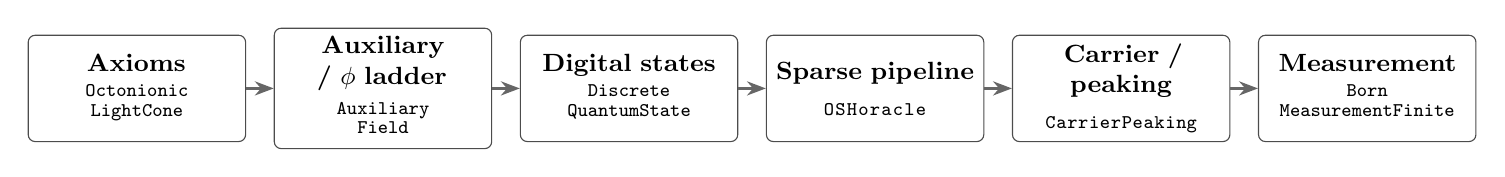
\begin{tikzpicture}[
  node distance=0.5cm and 0.35cm,
  box/.style={rectangle, draw=black!70, rounded corners=2.5pt, align=center, inner sep=3pt, minimum height=1.35cm, text width=2.55cm, font=\small},
  arr/.style={-{Stealth[length=2.4mm]}, thick, black!60}
]
\node[box] (ax) {\textbf{Axioms}\\[2pt]{\scriptsize\begin{tabular}{@{}c@{}}\lean{Octonionic}\\[-1pt]\lean{LightCone}\end{tabular}}};
\node[box, right=of ax] (aux) {\textbf{Auxiliary / }$\phi$\textbf{ ladder}\\[2pt]{\scriptsize\begin{tabular}{@{}c@{}}\lean{Auxiliary}\\[-1pt]\lean{Field}\end{tabular}}};
\node[box, right=of aux] (st) {\textbf{Digital states}\\[2pt]{\scriptsize\begin{tabular}{@{}c@{}}\lean{Discrete}\\[-1pt]\lean{QuantumState}\end{tabular}}};
\node[box, right=of st] (sp) {\textbf{Sparse pipeline}\\[2pt]{\scriptsize\lean{OSHoracle}}};
\node[box, right=of sp] (cp) {\textbf{Carrier / peaking}\\[2pt]{\scriptsize\lean{CarrierPeaking}}};
\node[box, right=of cp] (ms) {\textbf{Measurement}\\[2pt]{\scriptsize\begin{tabular}{@{}c@{}}\lean{Born}\\[-1pt]\lean{MeasurementFinite}\end{tabular}}};
\draw[arr] (ax) -- node[above, font=\scriptsize] {} (aux);
\draw[arr] (aux) -- (st);
\draw[arr] (st) -- (sp);
\draw[arr] (sp) -- (cp);
\draw[arr] (cp) -- (ms);
\end{tikzpicture}%
}
\caption{Lean-aligned pipeline (left to right). Variational layer: Section~\ref{sec:lagrangian}.}
\label{fig:roadmap}
\end{figure}

\section*{Acknowledgements}
The author acknowledges the use of AI-assisted development tools during manuscript and code production. In particular, Grok 4.20 and Composer 2 were used for programming assistance, Lean proof-development and verification support, and editorial revision support for manuscript drafting and refinement.

\section*{References}
\bibliographystyle{plain}
\bibliography{../references}

\end{document}
